\textbf{Agentic AI untuk Tata Kelola Data Kearsipan Konsisten dan
Terstruktur}

\textbf{Jatniko Nur Mutaqin*\textsuperscript{1)}, Ari Sandi Putra Ari
Tonang * \textsuperscript{1)}, Neng Ayu Herawati \textsuperscript{1)},
Lenny Putri Yulianty \textsuperscript{1)}, Kridanto Surendro
\textsuperscript{1)}}

\textsuperscript{1} Institut Teknologi Bandung, Bandung

Email: \textsuperscript{1}23523314@mahasiswa.itb.ac.id,
\textsuperscript{2}23523315@mahasiswa.itb.ac.id,

(Naskah masuk: dd mmm yyyy, diterima untuk diterbitkan: dd mmm yyyy)

\textbf{Abstrak}

Tata kelola data kearsipan konvensional sering menghadapi tantangan
terkait inkonsistensi penerapan kebijakan, metadata yang tidak
terstruktur, dan kesulitan dalam penegakan aturan secara konsisten.
Penelitian ini bertujuan untuk merancang dan mengusulkan sebuah model
konseptual berbasis Agentic AI guna mengatasi masalah tersebut secara
sistematis. Dengan menggunakan pendekatan \emph{Design Science Research}
(DSR) , penelitian ini menghasilkan sebuah arsitektur Sistem Multi-Agen
(MAS) yang holistik. Model ini terdiri dari serangkaian agen cerdas yang
otonom dan memiliki spesialisasi (misalnya, Agen Klasifikasi, Agen
Metadata, dan Agen Kepatuhan), yang dikoordinasikan oleh sebuah agen
orkestrator. Hasil utama menunjukkan bahwa pendekatan ini secara
fundamental mengubah paradigma tata kelola dari sekumpulan kebijakan
pasif menjadi logika aktif yang terintegrasi, dimana aturan-aturan
kearsipan dieksekusi secara otonom dan konsisten oleh seluruh agen.
Implementasi model ini diproyeksikan dapat meningkatkan konsistensi
proses, kualitas metadata secara signifikan, serta mendukung pencapaian
Indikator Kinerja Utama (IKU) kearsipan secara lebih objektif dan
terukur.

\textbf{Kata kunci}: Agentic AI, Indikator Kinerja Utama (IKU),
Kearsipan Digital, Sistem Multi-Agen, Tata Kelola Data

\textbf{Achieving Consistency and Structure in Archival Data Governance
through Agentic AI}

\emph{\textbf{Abstract}}

\emph{Conventional archival data governance often faces challenges
related to inconsistent policy implementation, unstructured metadata,
and difficulties in consistent rules enforcement. This research aims to
design and propose a conceptual model based on Agentic AI to
systematically address these issues. Employing a Design Science Research
(DSR) approach , this study develops a holistic Multi-Agent System (MAS)
architecture. This model comprises a suite of autonomous, specialized
intelligent agents (e.g., Classification Agent, Metadata Agent, and
Compliance Agent) , coordinated by an orchestrator agent. The primary
finding reveals that this approach fundamentally shifts the governance
paradigm from a set of passive policies to active, integrated logic ,
where archival rules are autonomously and consistently executed by the
agents. The implementation of this model is projected to significantly
enhance process consistency, improve metadata quality, and support the
achievement of archival Key Performance Indicators (KPIs) more
objectively and measurably}

\emph{\textbf{Keywords}: Agentic AI, Data Governance, Digital Archives,
Key Performance Indicators (KPIs), Multi-Agent System (MAS).}

\hypertarget{pendahuluan}{%
\section{\texorpdfstring{PENDAHULUAN
}{PENDAHULUAN }}\label{pendahuluan}}

Tata kelola data kearsipan yang efektif merupakan komponen fundamental
bagi operasional, akuntabilitas, dan keberlanjutan organisasi modern
(Maurel \& Zwarich, 2021). Berbagai studi dan praktik terbaik di bidang
manajemen informasi secara konsisten menekankan bahwa pengelolaan arsip
yang baik tidak hanya krusial untuk mendukung pengambilan keputusan
strategis berbasis bukti (Luo \& Hu, 2022; Tummers et al., 2020) dan
memastikan kepatuhan terhadap kerangka regulasi hukum yang berlaku
(Christiana et al., 2024; Kerpedzhiev et al., 2020), tetapi juga vital
dalam melestarikan memori kolektif serta aset intelektual organisasi
(Colavizza et al., 2022). Meskipun demikian, upaya untuk mencapai
implementasi tata kelola kearsipan yang optimal seringkali menghadapi
berbagai tantangan (Ma, 2024; Liu, 2024), terutama dalam sistem yang
masih mengandalkan proses manual atau semi-otomatis.

Masalah yang kerap diidentifikasi dalam literatur dan laporan praktik
meliputi potensi inkonsistensi dalam penerapan kebijakan dan prosedur
kearsipan antar unit kerja (Miller et al., 2020), yang dapat berakibat
pada pengelolaan arsip yang tidak seragam dan sulit diaudit. Standar dan
kebijakan yang jelas merupakan kunci untuk interoperabilitas (Magnuson
et al., 2020). Selain itu, terdapat kesulitan yang sering dilaporkan
dalam menjaga metadata arsip agar tetap terstruktur, lengkap, dan akurat
secara konsisten (Jones et al., 2023), padahal metadata berkualitas
tinggi merupakan prasyarat penting untuk temu kembali informasi yang
efisien dan andal. Kondisi ini dapat berimplikasi pada lambatnya proses
pencarian dan akses terhadap arsip yang dibutuhkan (Indrasweri et al.,
2022), dimana masalah ini berpotensi menghambat produktivitas dan
responsivitas organisasi. Dinamika kualitas sumber daya manusia (Massihi
et al., 2020) seringkali disebut sebagai faktor yang dapat memperberat
tantangan pengelolaan ini. Lebih lanjut, terdapat indikasi bahwa
berbagai tantangan dalam pengelolaan arsip ini dapat berkorelasi dengan
kesulitan organisasi dalam mencapai target kinerja tertentu (Luo \& Hu,
2022; Tripathi et al., 2020), meskipun hubungan kausal langsung dan
faktor-faktor kontributif lainnya memerlukan analisis yang lebih
mendalam pada setiap konteks organisasi.

Dalam menghadapi tantangan-tantangan tersebut, perkembangan teknologi
Kecerdasan Artifisial (AI), khususnya paradigma Agentic AI, mulai
dieksplorasi sebagai salah satu pendekatan yang berpotensi menawarkan
dukungan signifikan. Agentic AI, dengan karakteristiknya yang dirancang
untuk dapat bertindak secara otonom, proaktif, dan adaptif dalam
mencapai tujuan tertentu (Hosseini \& Seilani, 2025; Sapkota et al.,
2025), membuka peluang untuk merepresentasikan berbagai fungsi dan
proses krusial dalam tata kelola data kearsipan. Ini mencakup proses
mulai dari akuisisi, dukungan klasifikasi otomatis, manajemen metadata
cerdas (Shinde et al., 2024), hingga fasilitasi pemantauan kepatuhan
terhadap kebijakan, yang dapat diwujudkan sebagai serangkaian agen AI
yang bekerja secara terkoordinasi. Dengan mendelegasikan tugas-tugas
yang terdefinisi dengan baik dan seringkali repetitif kepada agen-agen
AI ini (Hajiyev, 2024), terdapat harapan untuk mencapai tingkat
konsistensi yang lebih tinggi dalam penerapan kebijakan dan prosedur,
serta menghasilkan struktur metadata yang lebih seragam, akurat, dan
berkualitas (Shinde et al., 2024).

Menyadari potensi transformatif ini, penelitian ini dirumuskan untuk
menjawab serangkaian pertanyaan fundamental. Pertama, bagaimana
arsitektur sistem berbasis Agentic AI dapat dirancang secara optimal
untuk merepresentasikan dan melaksanakan tugas-tugas kunci dalam tata
kelola data kearsipan, dengan fokus utama pada peningkatan konsistensi
penerapan kebijakan dan perbaikan struktur metadata. Kedua, sejauh mana
integrasi Agentic AI dalam proses ini berpotensi memberikan kontribusi
nyata terhadap pencapaian Indikator Kinerja Utama (IKU) kearsipan yang
lebih objektif dan terukur. Terakhir, apa saja faktor-faktor
kritis---termasuk tantangan implementasi praktis (Sapkota et al., 2025),
kebutuhan esensial akan supervisi manusia yang berkelanjutan, integrasi
yang tepat, serta desain yang cermat---yang perlu dipertimbangkan untuk
memastikan efektivitas dan akuntabilitas (Ackerman, 2025; Raza et al.,
2025) sistem Agentic AI dalam konteks tata kelola data kearsipan yang
lebih baik.

Sejalan dengan rumusan masalah tersebut, penelitian ini menetapkan
beberapa tujuan utama yang spesifik. Tujuan pertama adalah merancang dan
mengusulkan sebuah model konseptual arsitektur sistem berbasis Agentic
AI. Model ini diharapkan mampu merepresentasikan dan mengotomatiskan
tugas-tugas kunci dalam siklus tata kelola data kearsipan, sehingga
dapat secara langsung berkontribusi pada peningkatan konsistensi
penerapan kebijakan dan peningkatan kualitas struktur metadata.
Selanjutnya, penelitian ini bertujuan untuk menganalisis dan memetakan
secara komprehensif potensi kontribusi dari implementasi Agentic AI
terhadap peningkatan objektivitas dalam pengukuran dan IKU di bidang
kearsipan. Lebih lanjut, tujuan ketiga adalah mengidentifikasi dan
mengevaluasi secara kritis faktor-faktor pendukung dan penghambat, yang
mencakup aspek teknis, organisasional, serta kebutuhan intervensi
manusia dalam skema human-in-the-loop, guna memastikan penerapan Agentic
AI yang efektif dan akuntabel dalam tata kelola data kearsipan.

Diharapkan, penelitian ini akan memberikan manfaat yang signifikan baik
dari perspektif teoritis maupun praktis. Secara teoritis, penelitian ini
berpotensi memperkaya khazanah ilmu pengetahuan dalam disiplin manajemen
informasi, ilmu kearsipan, dan kecerdasan artifisial, terutama terkait
dengan aplikasi inovatif Agentic AI dalam konteks tata kelola data.
Selain itu, penelitian ini juga diharapkan dapat menyediakan kerangka
kerja konseptual baru untuk memahami bagaimana tugas-tugas kompleks
dalam tata kelola kearsipan dapat direpresentasikan dan diotomatisasi
secara efektif melalui arsitektur sistem berbasis agen AI. Dari sisi
praktis, manfaat yang diharapkan mencakup penyediaan panduan dan model
arsitektur yang dapat diadopsi oleh institusi kearsipan dan organisasi
lain dalam merancang serta mengimplementasikan solusi Agentic AI. Hal
ini bertujuan untuk meningkatkan efisiensi operasional, konsistensi
dalam pengelolaan, dan kualitas data kearsipan secara keseluruhan.
Penelitian ini juga diharapkan menawarkan wawasan bagi para pengambil
kebijakan dan praktisi kearsipan mengenai potensi Agentic AI dalam
mendukung pencapaian IKU dan meningkatkan tingkat akuntabilitas.
Terakhir, dengan mengidentifikasi faktor-faktor kunci yang perlu
diperhatikan, penelitian ini dapat membantu meminimalkan risiko dan
memaksimalkan dampak positif dari adopsi teknologi AI di bidang
kearsipan.

Untuk menjaga fokus dan kedalaman analisis, penelitian ini dibatasi oleh
beberapa aspek. Pertama, dalam hal fokus teknologi, penelitian ini
secara spesifik akan terkonsentrasi pada eksplorasi dan perancangan
model konseptual berbasis Agentic AI. Aspek teknis yang lebih mendalam,
seperti pemilihan algoritma spesifik atau pengembangan source code untuk
prototipe sistem secara penuh, berada di luar cakupan penelitian ini.
Kedua, dalam konteks tata kelola data, pembahasan akan difokuskan pada
aspek-aspek kearsipan yang secara langsung dapat direpresentasikan dan
didukung oleh agen AI. Ini meliputi proses akuisisi data, klasifikasi,
manajemen metadata, pemantauan kepatuhan terhadap kebijakan, dan
penyediaan layanan informasi dasar, serta keterkaitannya dengan IKU yang
relevan. Aspek tata kelola strategis pada tingkat tinggi atau kebijakan
organisasional yang lebih luas hanya akan disentuh sebatas relevansinya
dengan implementasi agen AI. Ketiga, evaluasi terhadap model konseptual
yang diusulkan akan lebih bersifat kualitatif dan analitis, didasarkan
pada prinsip-prinsip desain yang mapan dan analisis potensi dampaknya,
bukan melalui pengujian empiris berskala besar atau uji coba sistem
secara menyeluruh.

\hypertarget{kajian-pustaka}{%
\section{KAJIAN PUSTAKA}\label{kajian-pustaka}}

Literatur akademis dan standar industri secara konsisten menghadapi
tantangan-tantangan dalam tata kelola arsip digital yang telah diuraikan
pada bagian Pendahuluan. Untuk mengatasi tantangan tersebut, kerangka
kerja seperti ISO 15489:2016 menjadi acuan fundamental yang menetapkan
prinsip-prinsip untuk manajemen arsip yang akuntabel, termasuk
penciptaan, penggunaan, pemeliharaan, dan disposisi arsip.
Prinsip-prinsip ini menekankan pentingnya arsip yang otentik, andal,
utuh, dan dapat digunakan. Namun, penerapan prinsip-prinsip ini secara
konsisten di lingkungan digital yang kompleks dan bervolume besar tetap
menjadi hambatan utama, yang mendorong perlunya eksplorasi solusi
teknologi inovatif.

\hypertarget{paradigma-agentic-ai-dan-sistem-multi-agen-mas}{%
\paragraph{2.2 Paradigma Agentic AI dan Sistem Multi-Agen
(MAS)}\label{paradigma-agentic-ai-dan-sistem-multi-agen-mas}}

Untuk menjawab kebutuhan akan solusi yang lebih dinamis dan otonom,
penelitian ini berfokus pada paradigma Agentic AI. Berbeda dengan AI
konvensional yang reaktif, Agentic AI dirancang untuk bertindak secara
proaktif dan adaptif guna mencapai tujuan yang kompleks. Arsitektur yang
umum digunakan untuk implementasinya adalah Sistem Multi-Agen (MAS), di
mana sistem terdiri dari beberapa agen cerdas yang berkolaborasi.

Menurut literatur teknis, arsitektur MAS yang efektif memiliki beberapa
komponen kunci: (a) Agen-agen Spesialis: Entitas otonom yang memiliki
keahlian khusus (misalnya, analisis data, validasi kepatuhan). (b) Agen
Koordinator/Orkestrator: Pengatur alur kerja yang mendelegasikan tugas
dan mengelola interaksi antar-agen (c) Basis Pengetahuan Bersama:
Repositori aturan, model, dan kebijakan yang dapat diakses oleh semua
agen untuk memastikan konsistensi dalam pengambilan keputusan.

Pendekatan arsitektural ini telah terbukti berhasil mengotomatisasi
proses kompleks di domain lain seperti keuangan dan logistik, dan
menawarkan potensi besar untuk diterapkan pada tata kelola kearsipan.

\hypertarget{peta-penelitian-ai-dalam-kearsipan-dan-celah-yang-ada}{%
\paragraph{2.3 Peta Penelitian AI dalam Kearsipan dan Celah yang
Ada}\label{peta-penelitian-ai-dalam-kearsipan-dan-celah-yang-ada}}

Penerapan AI dalam ilmu kearsipan cenderung bersifat terpisah. Tinjauan
sistematis dan studi kasus dari lembaga arsip menunjukkan bahwa AI lebih
banyak digunakan sebagai alat untuk tugas-tugas spesifik
(\emph{task-specific}), seperti klasifikasi otomatis, ekstraksi
metadata, atau dukungan akses informasi.

Meskipun penelitian terdahulu telah mengeksplorasi penggunaan agen untuk
pelestarian digital, terdapat celah penelitian yang jelas: belum adanya
model arsitektur terintegrasi yang menerapkan paradigma MAS modern untuk
mengelola keseluruhan siklus hidup tata kelola kearsipan, mulai dari
akuisisi hingga pemantauan IKU secara berkelanjutan. Penelitian ini
dirancang untuk mengisi celah tersebut dengan mengusulkan model
konseptual yang holistik.

\hypertarget{metode-penelitian}{%
\section{METODE PENELITIAN}\label{metode-penelitian}}

Penelitian ini menerapkan pendekatan \emph{Design Science Research}
(DSR) untuk menghasilkan artefak utama berupa model konseptual
arsitektur Agentic AI. Fokus DSR dalam konteks ini adalah pada
perancangan solusi inovatif untuk meningkatkan konsistensi dan struktur
dalam tata kelola data kearsipan.

Pengembangan model ini didasarkan pada sintesis kritis dari sumber data
sekunder yang komprehensif. Sumber utama meliputi: (1) Literatur ilmiah
terkini (jurnal, prosiding, buku) mengenai tata kelola kearsipan,
Agentic AI, Multi-Agent Systems, dan IKU kearsipan; (2) Standar
internasional relevan (khususnya seri ISO 15489) dan dokumen kebijakan
terkait; serta (3) Laporan praktik dan studi kasus publikasi mengenai
implementasi sistem informasi atau AI di organisasi.

Pengumpulan data dilakukan melalui dua teknik utama: (1) Studi literatur
sistematis terfokus untuk mengidentifikasi landasan teoritis, praktik
terbaik, dan lanskap teknologi Agentic AI yang relevan; dan (2) Analisis
dokumen kualitatif terhadap standar dan laporan untuk mengekstrak
persyaratan fungsional, kriteria IKU, dan konteks implementasi.

Proses perancangan artefak model konseptual melibatkan identifikasi
komponen agen AI kunci yang merepresentasikan fungsi tata kelola
kearsipan, pendefinisian fungsionalitas dan interaksi antar agen, serta
pemetaan alur kerja yang didukung oleh agen-agen tersebut.
Prinsip-prinsip desain sistem cerdas dan tata kelola AI yang bertanggung
jawab menjadi acuan dalam perancangan.

Evaluasi model konseptual dilakukan secara analitis dan kualitatif. Ini
mencakup demonstrasi potensi model melalui skenario kasus penggunaan
ilustratif, pemetaan model terhadap kriteria desain yang diturunkan dari
literatur, serta analisis potensi kontribusinya terhadap IKU kearsipan
dan identifikasi faktor-faktor implementasi kritis.

\hypertarget{hasil-dan-analisis}{%
\section{HASIL DAN ANALISIS}\label{hasil-dan-analisis}}

\hypertarget{kapabilitas-agentic-ai-untuk-tata-kelola-kearsipan}{%
\subsection{4.1. Kapabilitas Agentic AI untuk Tata Kelola
Kearsipan}\label{kapabilitas-agentic-ai-untuk-tata-kelola-kearsipan}}

Transformasi tata kelola data kearsipan menuju sistem yang lebih
konsisten, terstruktur, dan efisien dapat secara signifikan didukung
oleh pemanfaatan kapabilitas kunci yang inheren dalam paradigma Agentic
AI. Analisis mendalam mengidentifikasi beberapa kapabilitas fundamental
yang paling relevan dan berpotensi memberikan dampak transformatif, yang
akan diuraikan sebagai berikut:

\begin{enumerate}
\def\labelenumi{\arabic{enumi}.}
\item
  \textbf{Otonomi Terarah}
\end{enumerate}

Deskripsi Kapabilitas: Agen AI dirancang untuk beroperasi secara mandiri
dalam batas-batas dan tujuan yang telah ditetapkan oleh manusia
(arsiparis atau administratorzy sistem). Agen ini dapat menjalankan
serangkaian tugas tanpa intervensi langsung untuk setiap langkah, namun
tetap bekerja menuju sasaran spesifik yang telah dikonfigurasikan,
seperti penerapan skema klasifikasi atau validasi kelengkapan metadata.

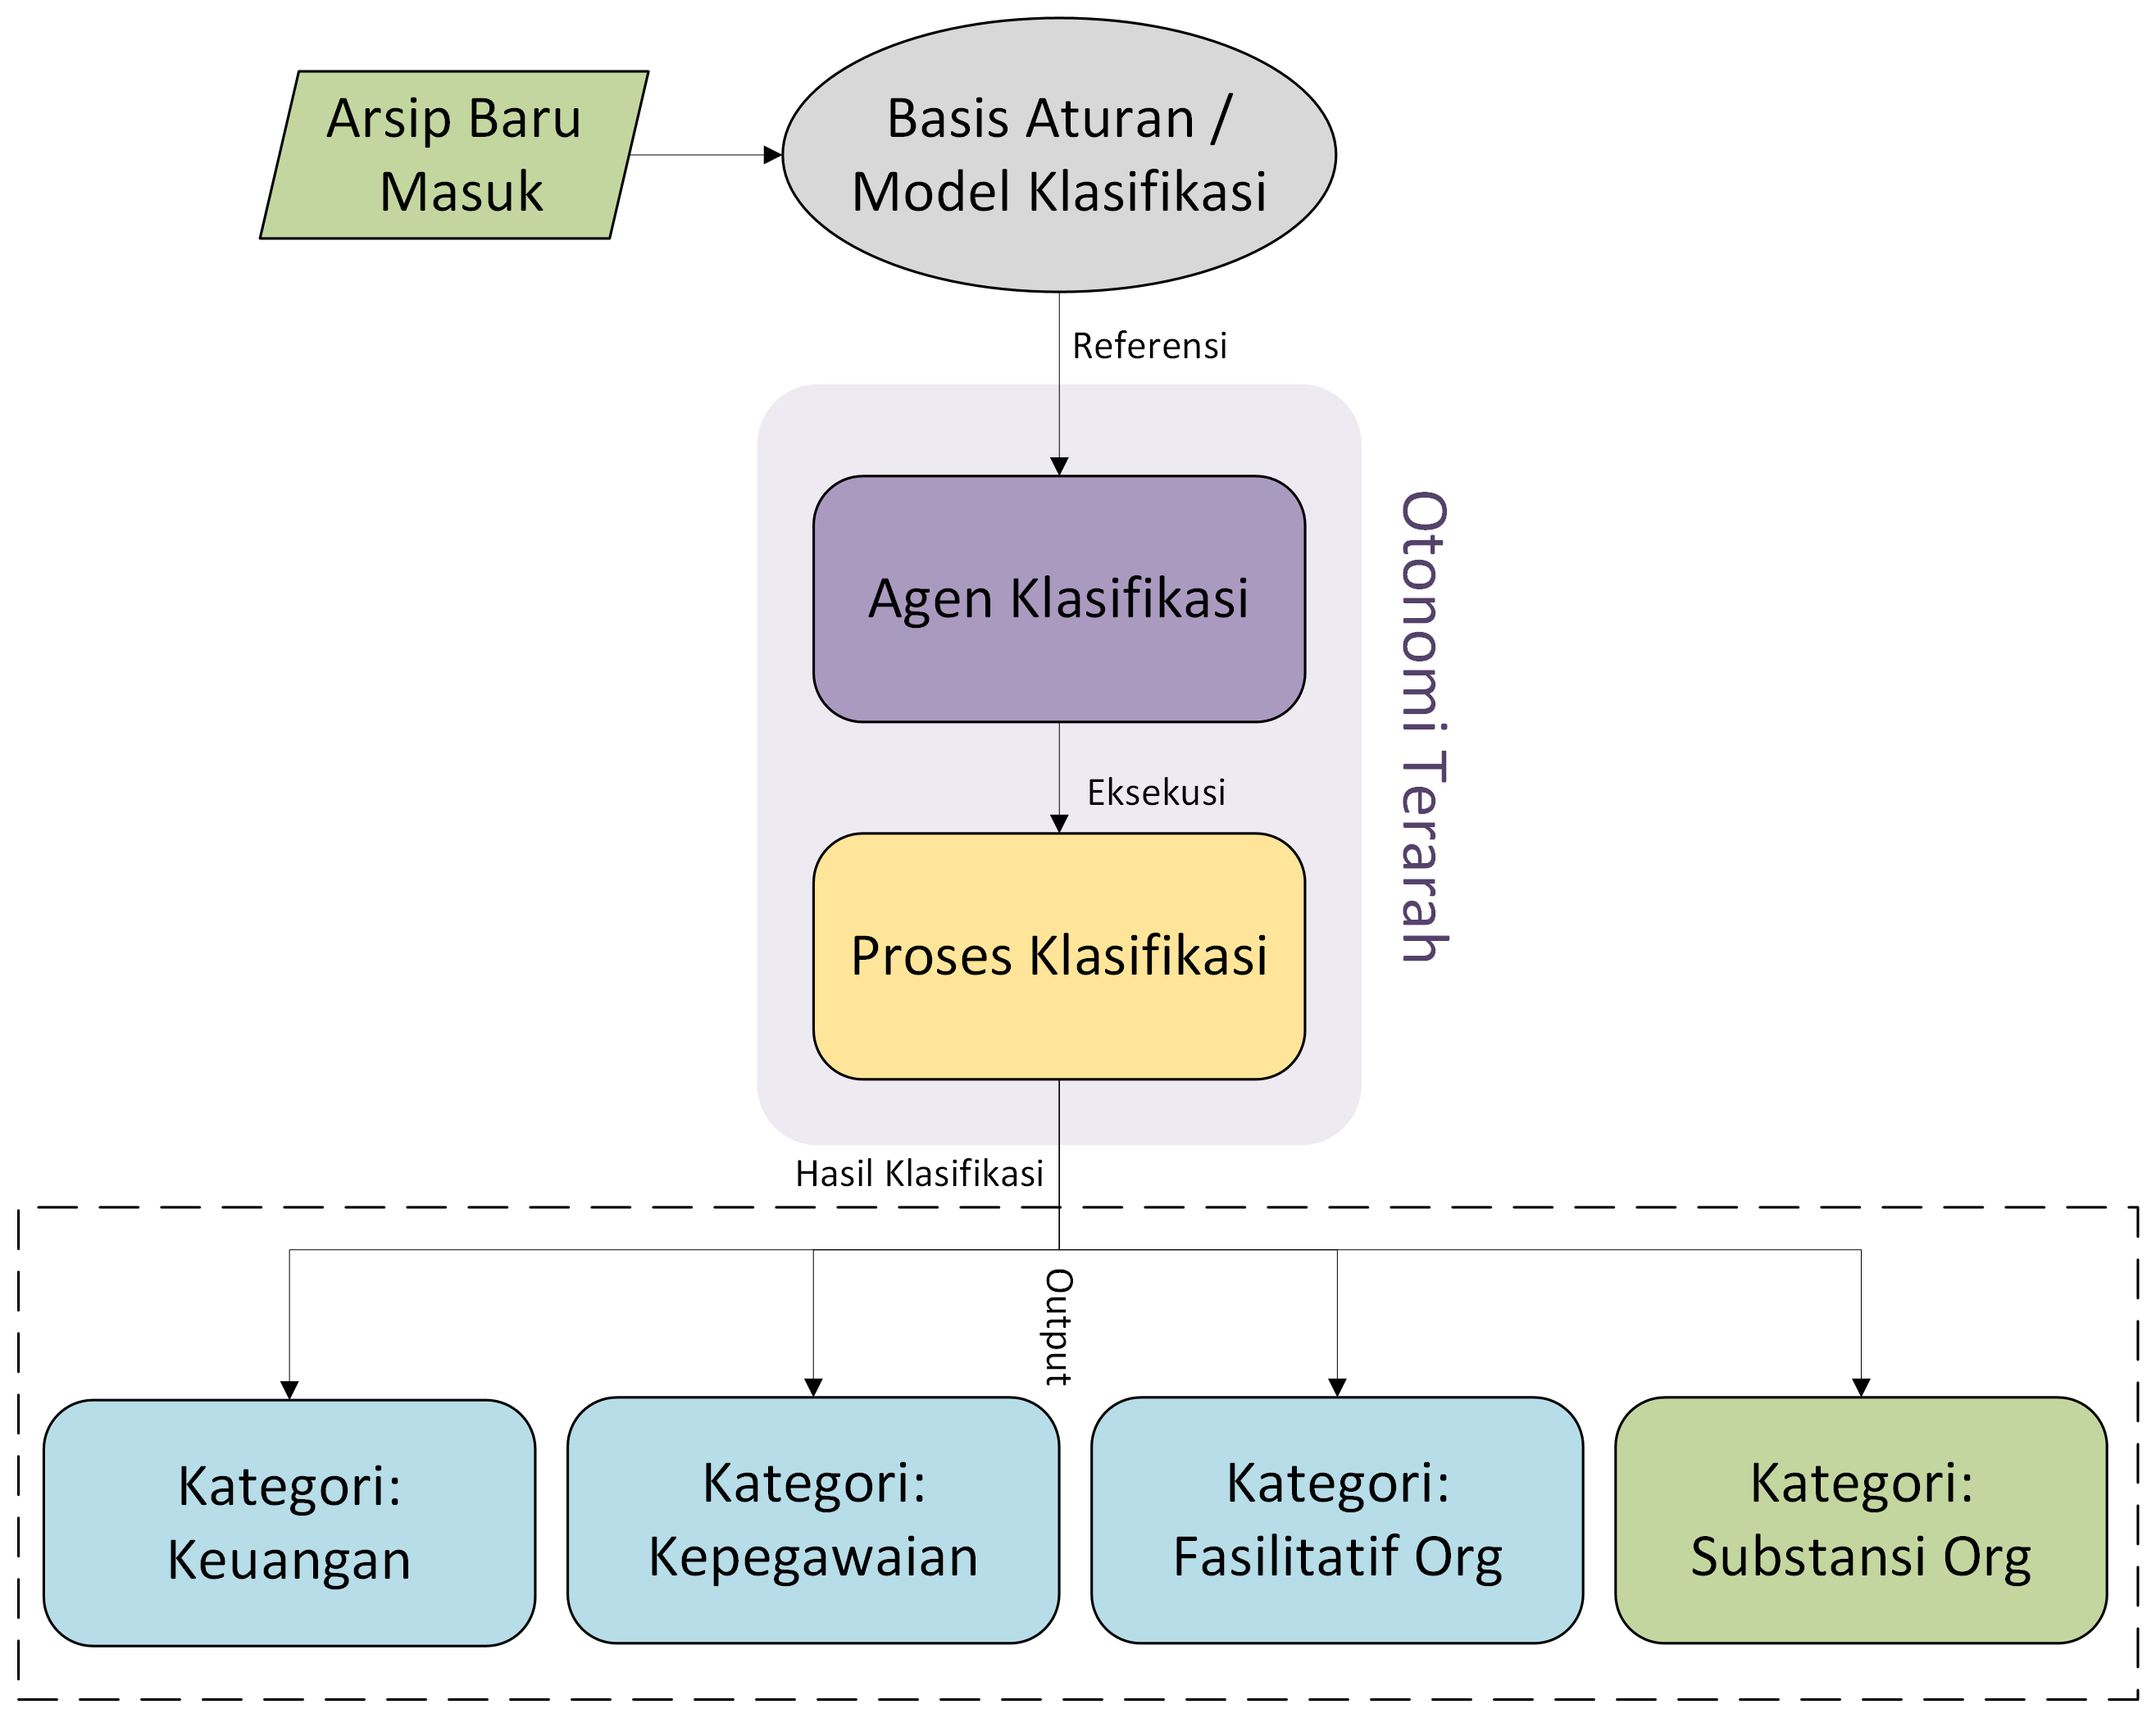
\includegraphics[width=3.21319in,height=2.80278in]{media/media/image1.png}

Gambar 1. Contoh Agen Otonom Menerapkan Aturan Klasifikasi

Relevansi untuk tata kelola kearsipan: (1) Konsistensi Proses: Dengan
otonomi terarah, agen AI dapat secara konsisten menerapkan kebijakan dan
prosedur kearsipan yang sama pada setiap arsip atau transaksi data,
mengurangi variabilitas yang sering muncul akibat interpretasi manusia
yang berbeda atau kelelahan. Misalnya, agen dapat secara otonom
menerapkan aturan penamaan file standar atau mengalokasikan arsip ke
folder yang tepat berdasarkan aturan klasifikasi. (2) Kemampuan untuk
bekerja secara otonom memungkinkan penanganan volume data kearsipan yang
besar secara efisien, tugas yang seringkali membebani sumber daya
manusia.

\begin{enumerate}
\def\labelenumi{\arabic{enumi}.}
\setcounter{enumi}{1}
\item
  \textbf{Proaktivitas Berbasis Aturan dan Tujuan}
\end{enumerate}

Deskripsi Kapabuilitas: Berbeda dengan sistem yang hanya reaktif,
Agentic AI dapat mengambil inisiatif untuk bertindak guna mencapai
tujuannya atau berdasarkan aturan yang telah diprogram. Agen tidak hanya
menunggu perintah, tetapi dapat memicu tindakan berdasarkan kondisi
tertentu atau untuk mencegah masalah potensial.

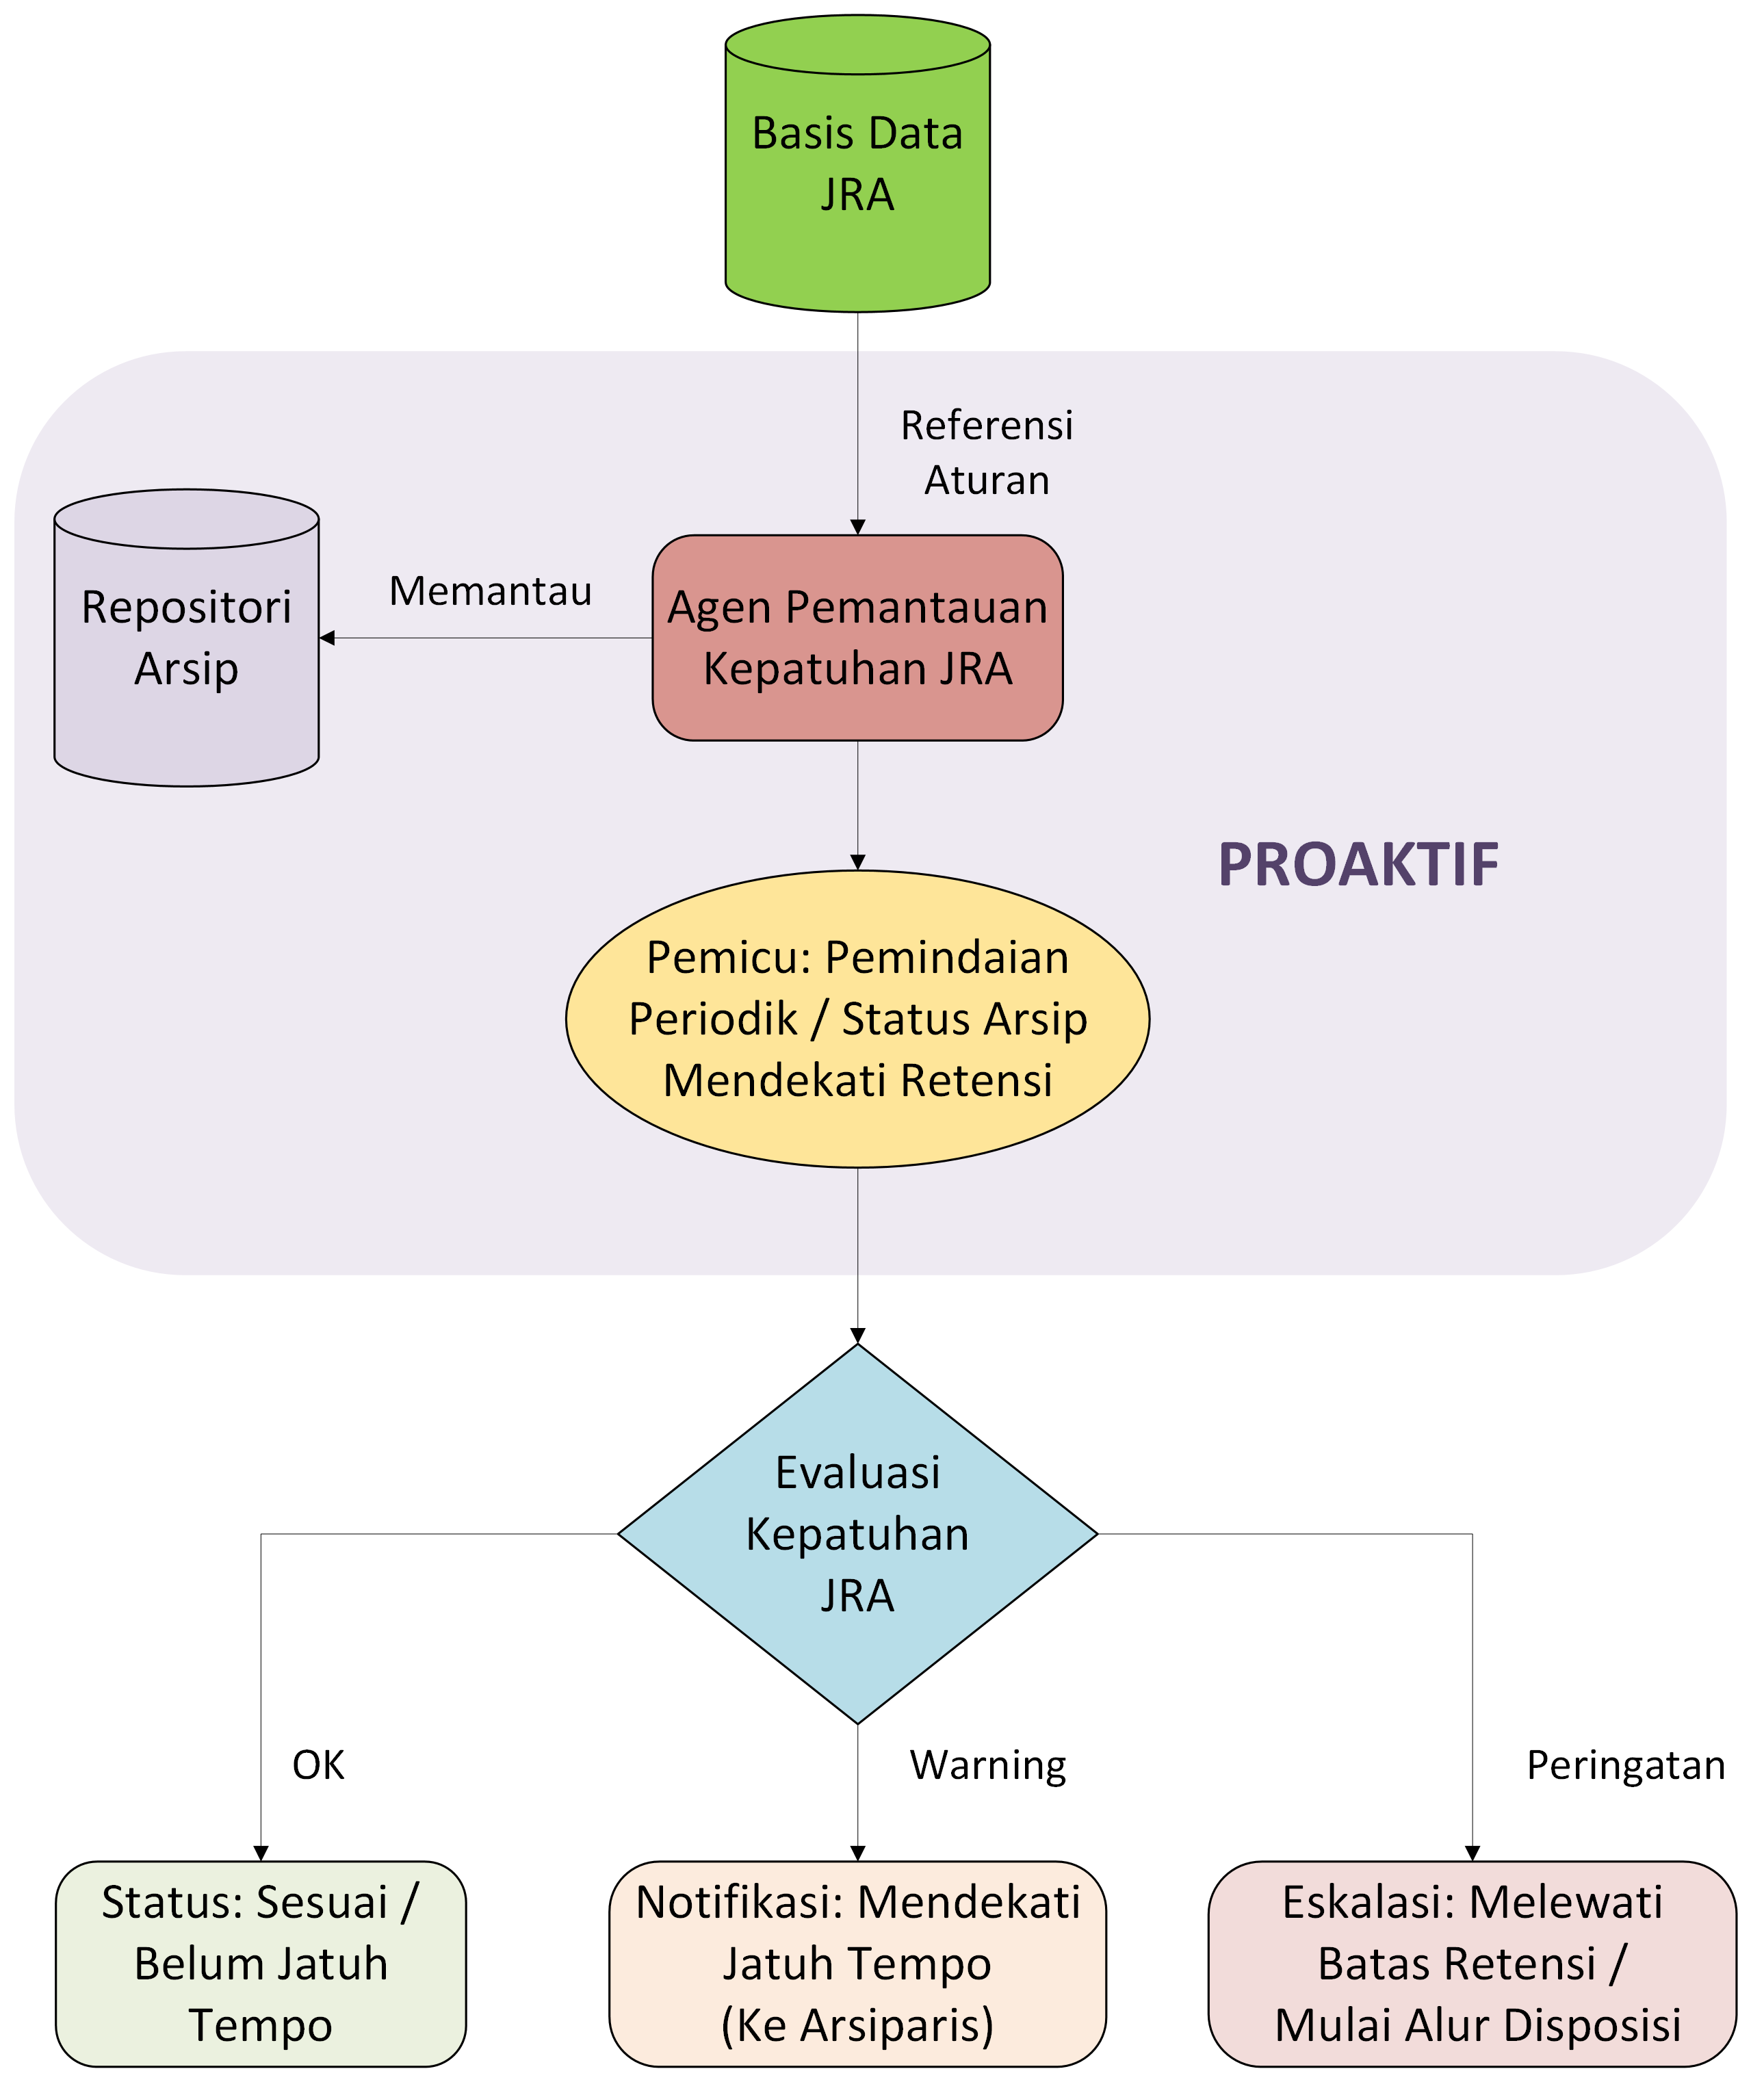
\includegraphics[width=3.05139in,height=3.62431in]{media/media/image2.png}

Gambar 2. Agen proaktif memantau kepatuhan standar metadata

Relevansi untuk tata kelola kearsipan: (1) Pemantauan Kepatuhan Aktif:
Agen AI dapat secara proaktif memantau kepatuhan terhadap jadwal retensi
arsip, kebijakan keamanan, atau standar metadata. Jika terdeteksi
potensi pelanggaran atau ketidaksesuaian (misalnya, metadata yang hilang
setelah periode waktu tertentu), agen dapat secara otomatis memberikan
notifikasi, memulai alur kerja perbaikan, atau bahkan melakukan tindakan
korektif sederhana. (2) Identifikasi Risiko Dini: Agen dapat dilatih
untuk mengenali pola yang mengindikasikan risiko terhadap integritas
atau keamanan arsip, dan secara proaktif mengambil langkah mitigasi atau
memberi tahu penanggung jawab.(3) Pemeliharaan Struktur Data: Agen dapat
proaktif memeriksa dan memperbaiki inkonsistensi dalam struktur metadata
atau skema klasifikasi secara berkala.

\begin{enumerate}
\def\labelenumi{\arabic{enumi}.}
\setcounter{enumi}{2}
\item
  \textbf{Kemampuan Belajar dan Adaptasi}
\end{enumerate}

Deskripsi Kapabilitas: Agentic AI (terutama yang memanfaatkan machine
learning) memiliki kemampuan untuk belajar dari data baru, interaksi,
dan umpan balik (\emph{feedback}) untuk meningkatkan kinerjanya seiring
waktu. Agen dapat beradaptasi dengan perubahan pola data atau kebutuhan
pengguna.

Relevansi untuk tata kelola kearsipan: (1) Peningkatan Akurasi
Klasifikasi dan Ekstraksi Metadata: Melalui mekanisme
\emph{Human-in-the-Loop} (HITL), agen AI dapat belajar dari koreksi yang
dilakukan oleh arsiparis, sehingga saran klasifikasi atau ekstraksi
metadata otomatis menjadi semakin akurat. (2) Adaptasi terhadap
Perubahan Kebijakan: Meskipun memerlukan konfigurasi ulang, agen yang
adaptif dapat lebih mudah disesuaikan untuk mengikuti perubahan dalam
kebijakan kearsipan atau standar metadata daripada melakukan perubahan
manual pada seluruh sistem. (3) Optimasi Proses: Agen dapat belajar
mengidentifikasi \emph{bottleneck} atau inefisiensi dalam alur kerja
kearsipan dan menyarankan atau mengimplementasikan optimasi.

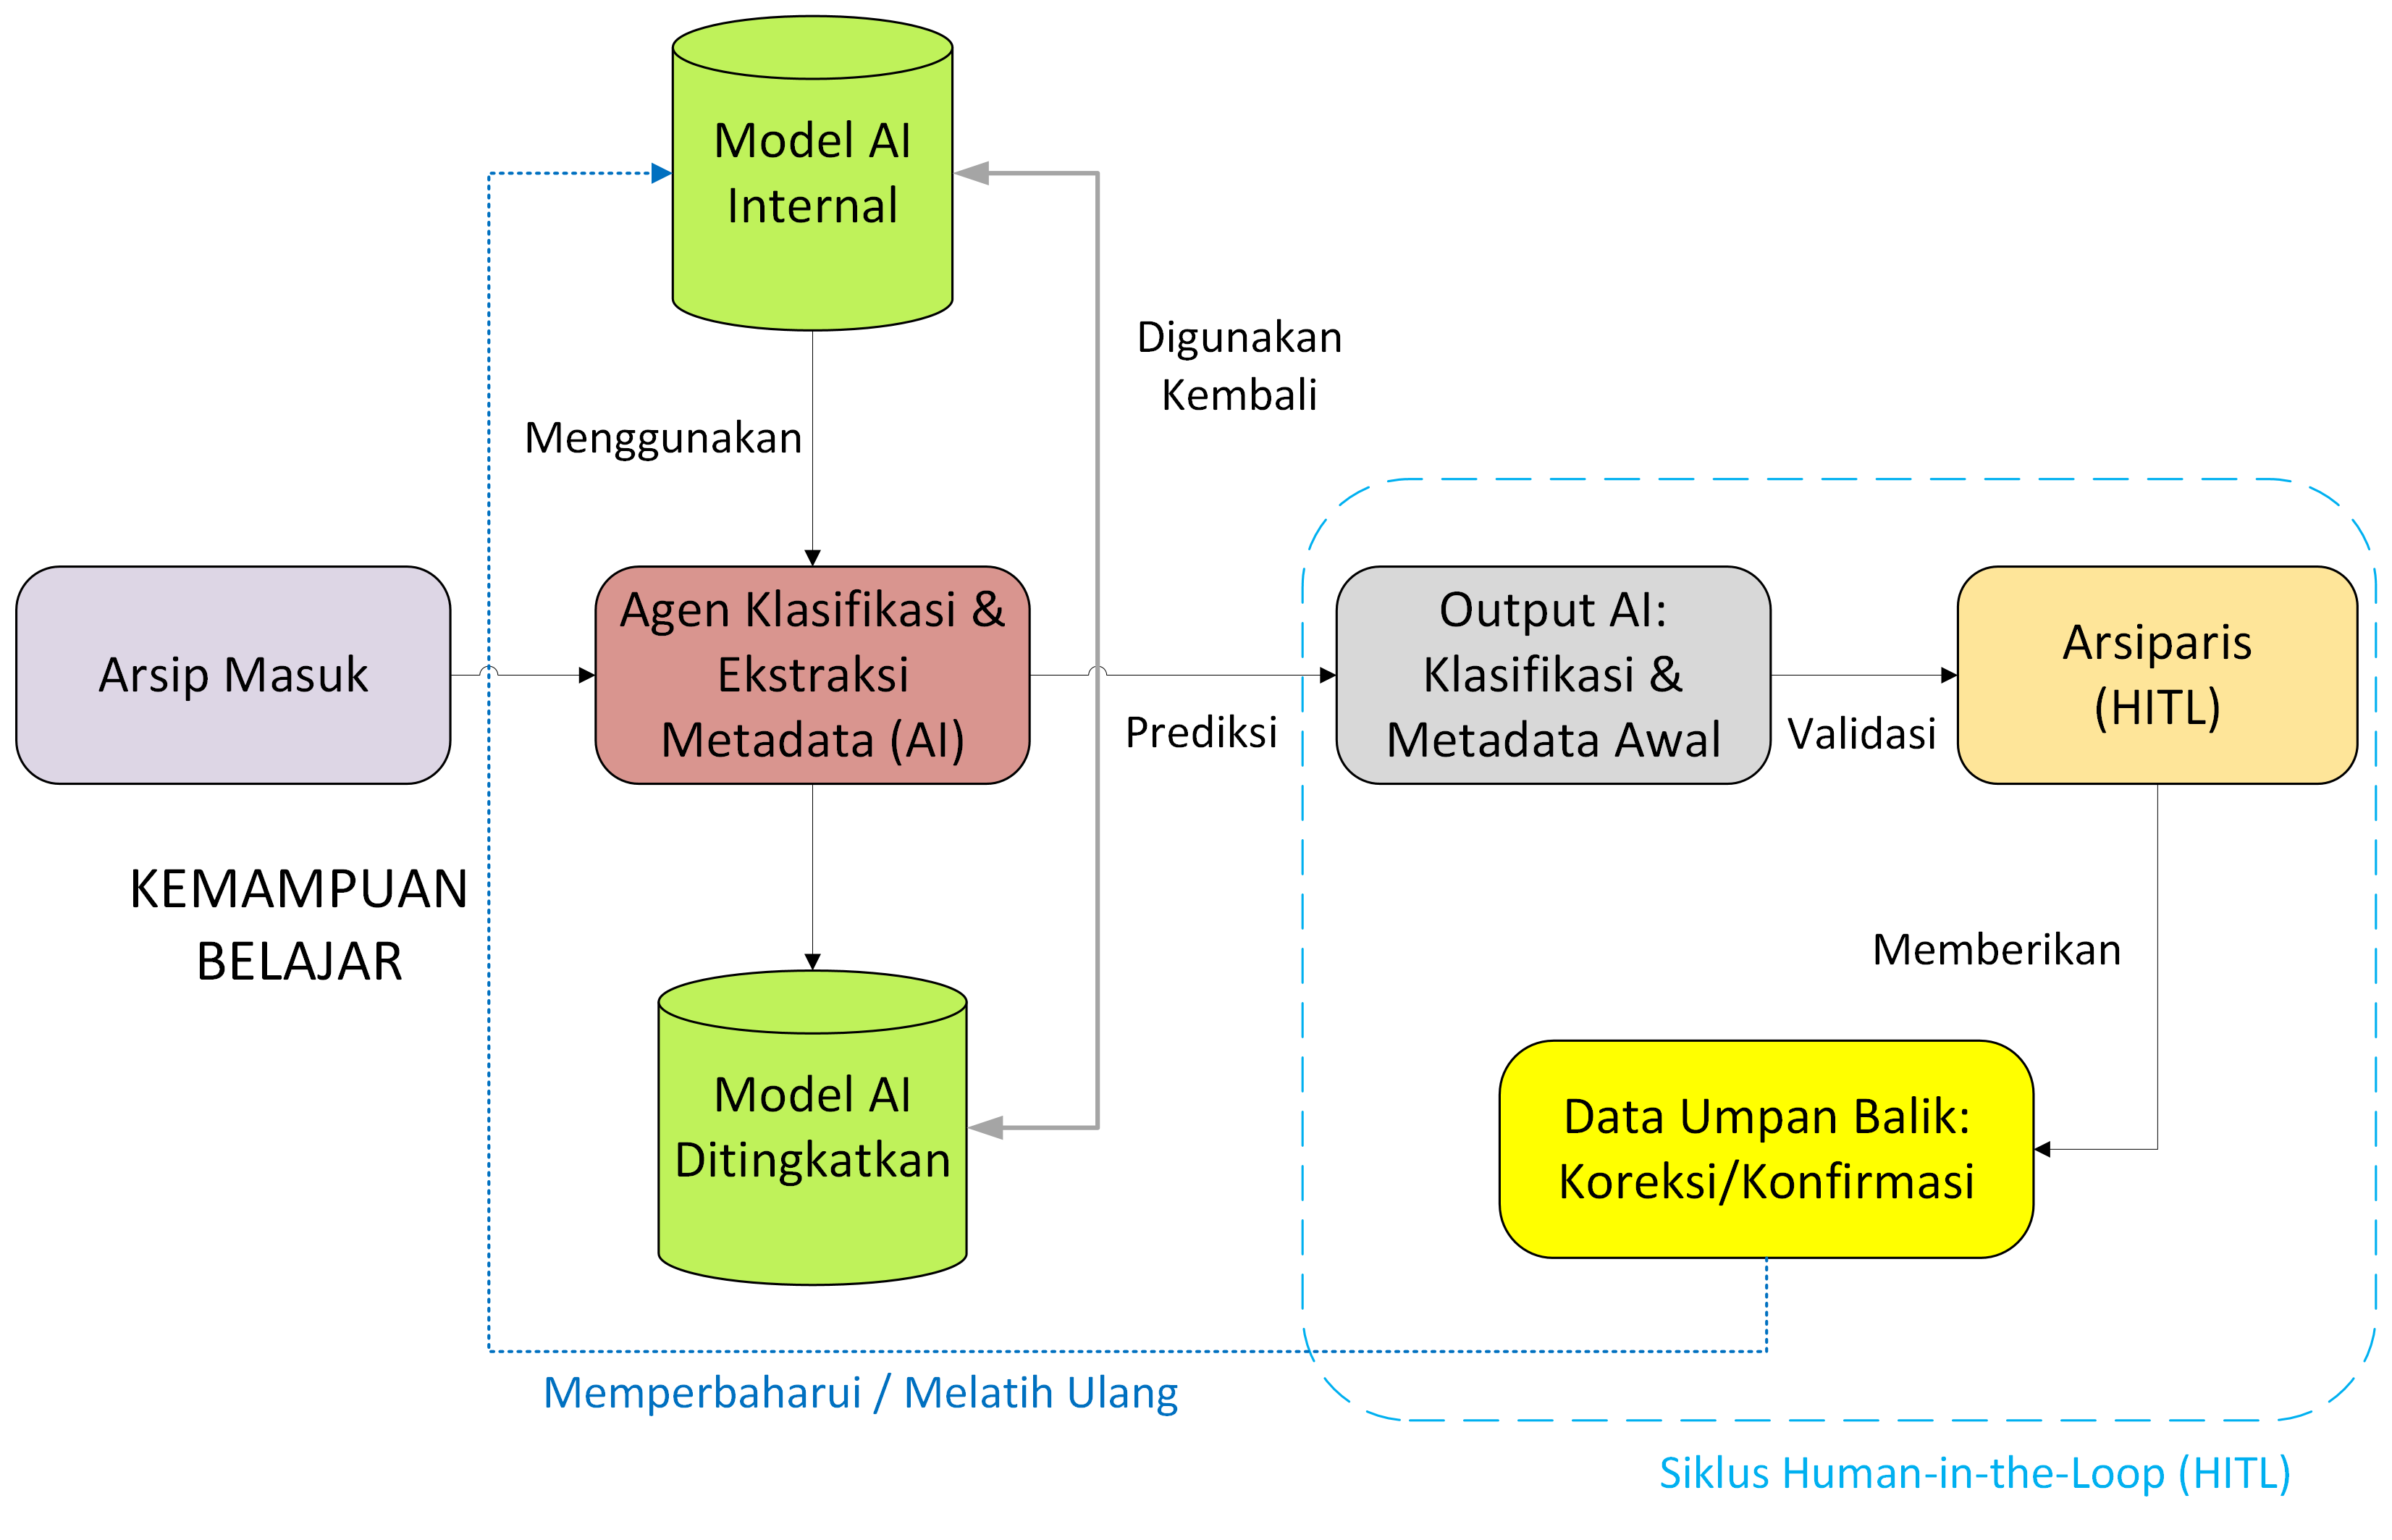
\includegraphics[width=2.99386in,height=1.92708in]{media/media/image3.png}

Gambar 3. Agen Pembelajar dengan Mekanisme HITL untuk Meningkatkan
Akurasi Klasifikasi \& Ekstraksi Metadata

\textbf{4.1.4 Koordinasi dan Kolaborasi dalam Sistem Multi-Agen}

Deskripsi Kapabuilitas: Agentic AI diimplementasikan dalam arsitektur
Multi-Agent System (MAS), di mana berbagai agen dengan spesialisasi
berbeda bekerja sama untuk mencapai tujuan yang lebih besar. Agen dapat
berkomunikasi, bernegosiasi, dan mengoordinasikan tindakan. Relevansi
untuk tata kelola kearsipan: (1) Pembagian Kerja yang Efisien:
Tugas-tugas kompleks dalam tata kelola kearsipan (misalnya, mulai dari
akuisisi hingga disposisi) dapat dipecah dan didelegasikan ke agen-agen
spesialis (misalnya, Agen Akuisisi, Agen Metadata, Agen Retensi, Agen
Layanan). (2) Alur Kerja Terotomatisasi dan Terintegrasi: Agen-agen
dapat saling memicu tindakan secara berurutan atau paralel, menciptakan
alur kerja tata kelola yang terotomatisasi. Contohnya, setelah Agen
Akuisisi mendaftarkan arsip baru, Agen dapat memberi sinyal kepada Agen
Metadata untuk memulai proses ekstraksi dan validasi metadata. (3)
Peningkatan Konsistensi Lintas Fungsi: Dengan agen-agen yang beroperasi
berdasarkan aturan dan tujuan bersama dalam MAS, konsistensi dapat
dijaga tidak hanya dalam satu tugas, tetapi juga lintas berbagai fungsi
tata kelola kearsipan.

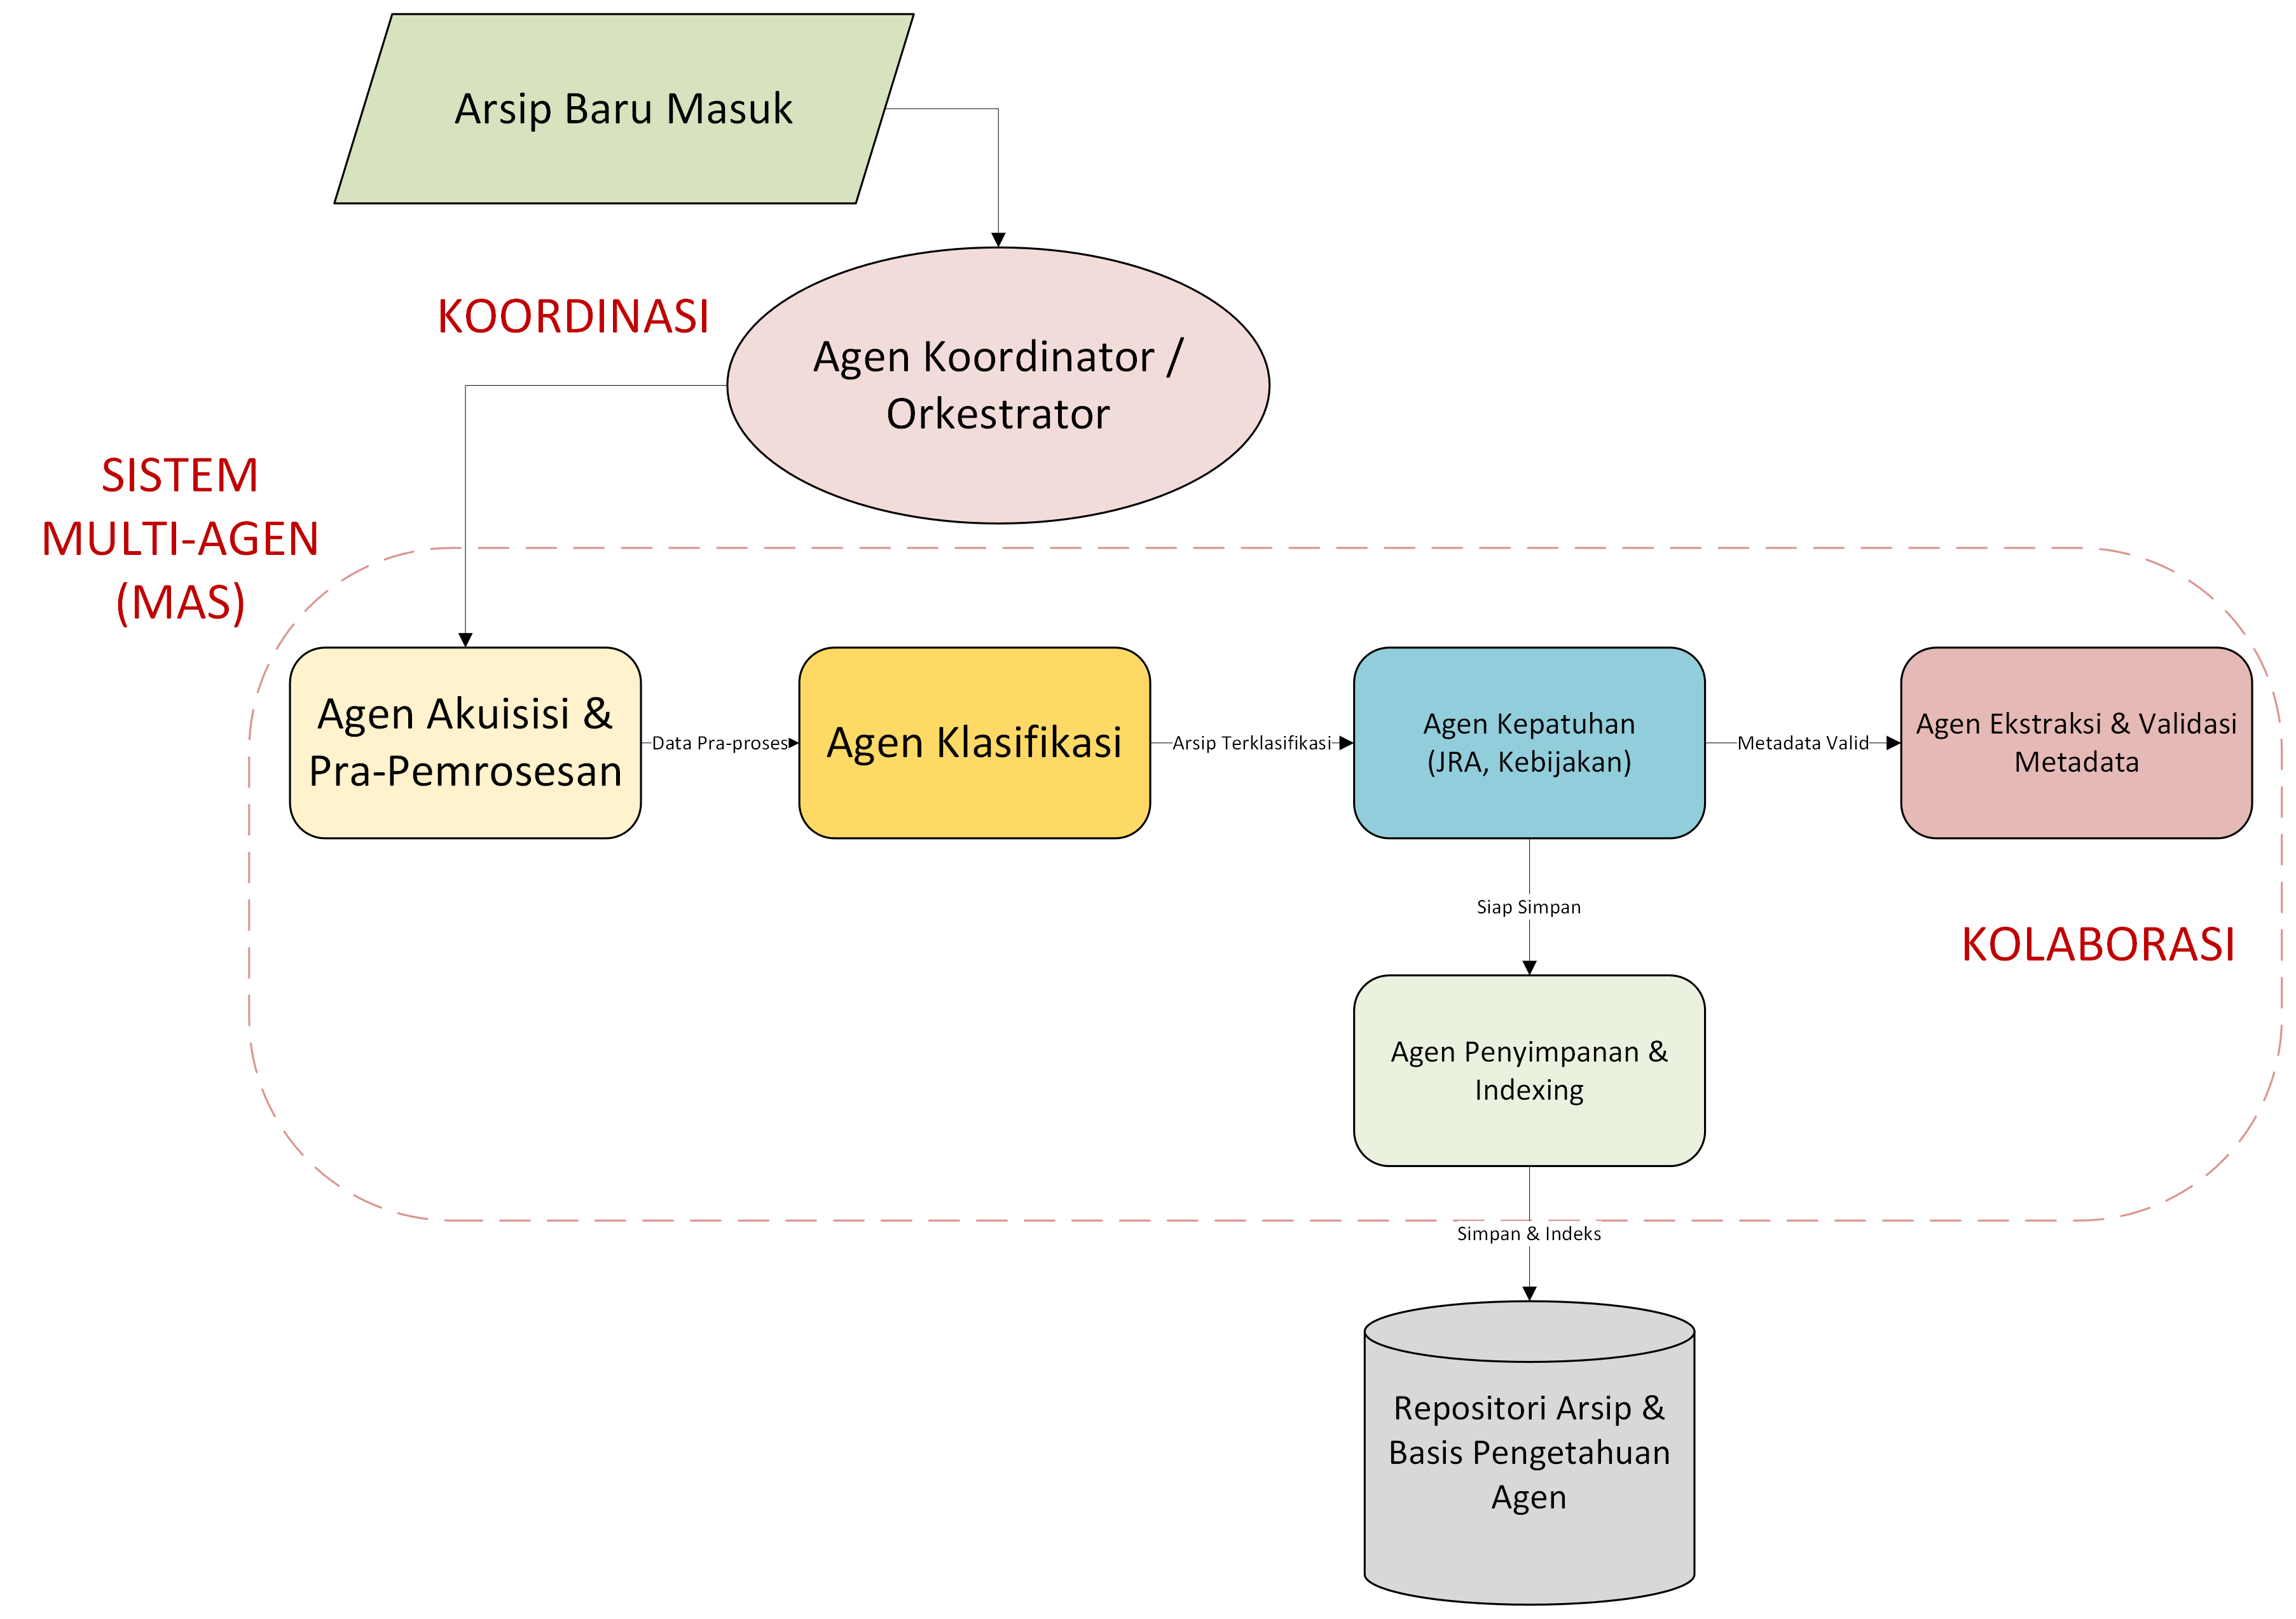
\includegraphics[width=2.9in,height=2.04583in]{media/media/image4.png}

Gambar 4. Sistem Multi Agen dalam Tata Kelola Data Kearsipan

\textbf{4.2. Kontribusi Agentic AI terhadap IKU}

\hypertarget{implementasi-arsitektur-sistem-multi-agen-mas-berbasis-agentic-ai-sebagaimana-diusulkan-dalam-penelitian-ini-diproyeksikan-memberikan-kontribusi-signifikan-dan-positif-terhadap-pencapaian-berbagai-iku-yang-menjadi-tolak-ukur-keberhasilan-tata-kelola-kearsipan.-dengan-kemampuan-otomatisasi-cerdas-peningkatan-konsistensi-dan-pemrosesan-data-yang-lebih-akurat-sistem-ini-berpotensi-meningkatkan-skor-iku-di-berbagai-aspek-fundamental.}{%
\subsection{Implementasi arsitektur Sistem Multi-Agen (MAS) berbasis
Agentic AI sebagaimana diusulkan dalam penelitian ini diproyeksikan
memberikan kontribusi signifikan dan positif terhadap pencapaian
berbagai IKU yang menjadi tolak ukur keberhasilan tata kelola kearsipan.
Dengan kemampuan otomatisasi cerdas, peningkatan konsistensi, dan
pemrosesan data yang lebih akurat, sistem ini berpotensi meningkatkan
skor IKU di berbagai aspek
fundamental.}\label{implementasi-arsitektur-sistem-multi-agen-mas-berbasis-agentic-ai-sebagaimana-diusulkan-dalam-penelitian-ini-diproyeksikan-memberikan-kontribusi-signifikan-dan-positif-terhadap-pencapaian-berbagai-iku-yang-menjadi-tolak-ukur-keberhasilan-tata-kelola-kearsipan.-dengan-kemampuan-otomatisasi-cerdas-peningkatan-konsistensi-dan-pemrosesan-data-yang-lebih-akurat-sistem-ini-berpotensi-meningkatkan-skor-iku-di-berbagai-aspek-fundamental.}}

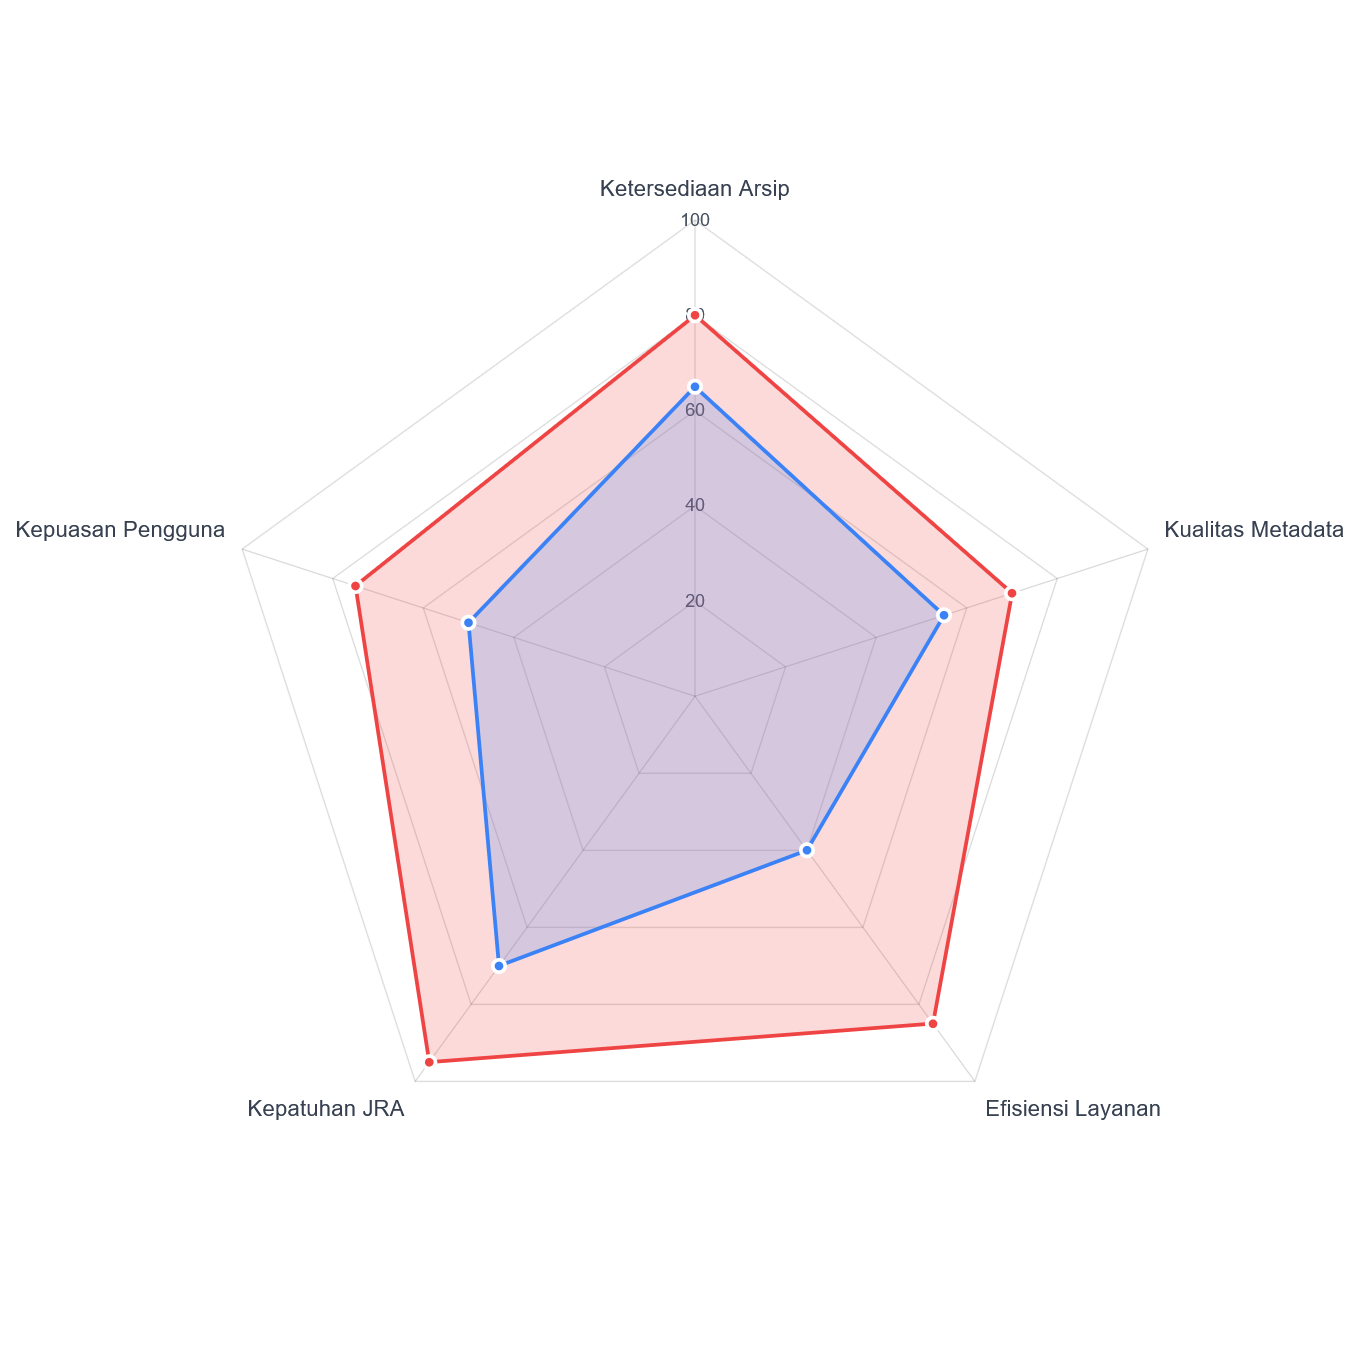
\includegraphics[width=2.57722in,height=1.92486in]{media/media/image5.png}

Gambar 5. Proyeksi peningkatan skor IKU dari Pemanfaatan Agentic AI

Terdapat lima IKU yang menjadi target penerapan Agentic AI tata kelola
data ini, yaitu: (a) Ketersediaan dan Aksesibilitas Arsip, (b) Kualitas
metadata dan struktur infomasi, Efisiensi Layanan informasi kearsipan.
(c) kepatuhan terhadap regulasi dan kebijakan, serta Efisiensi
Operasional dan Tata Kelola Secara Umum

\textbf{4.2.1 IKU Ketersediaan dan Aksesibilitas Arsip}

IKU yang relevan berfokus pada dua area utama yaitu efisiensi pengolahan
dan kecepatan akses arsip. Untuk IKU terkait pengolahan seperti
mengurangi backlog dan melengkapi deskripsi arsip, diperlukan Agentic AI
yang mampu mengotomatisasi proses akuisisi, klasifikasi, dan ekstraksi
metadata. Sementara itu, untuk IKU terkait akses seperti mempercepat
waktu temu kembali informasi, dibutuhkan agen AI yang unggul dalam
indexing cerdas dan layanan pencarian instan.

Tabel 1: Proyeksi Kontribusi Agentic AI terhadap IKU ketersediaan dan
Aksesibilitas Arsip


\includegraphics[width=2.9in,height=3.33125in]{media/media/image6.emf}

\textbf{4.2.2 IKU Kualitas Metadata dan Struktur Informasi}

IKU yang relevan secara spesifik menargetkan berbagai aspek peningkatan
kualitas metadata, mulai dari kelengkapan, akurasi, konsistensi
penggunaan skema, hingga pemenuhan standar interoperabilitas.

Untuk mencapai hal ini, hubungan dengan Agentic AI sangatlah krusial, di
mana peran utama dipegang oleh Agen Ekstraksi \& Validasi Metadata untuk
mengotomatiskan pengisian dan pemeriksaan data. Kinerjanya kemudian
disempurnakan oleh Agen Pembelajar (HITL) yang terus meningkatkan
akurasi, serta agen lain yang menjamin penggunaan skema dan standar
secara konsisten.

Tabel 2: Proyeksi Kontribusi Agentic AI terhadap IKU Kualitas metadata
dan struktur informasi


\includegraphics[width=2.9in,height=3.00278in]{media/media/image7.emf}

\textbf{4.2.3 IKU Efisiensi Layanan Informasi Kearsipan}

IKU yang relevan berpusat pada peningkatan kualitas layanan pengguna,
yang diukur dari kecepatan respons, tingkat kepuasan, hingga kemampuan
pengguna untuk melakukan layanan mandiri (self-service). Untuk memenuhi
target ini, hubungan dengan Agentic AI sangatlah vital, dengan Agen
Layanan Cerdas sebagai komponen utama yang berfungsi sebagai garda
terdepan untuk interaksi pengguna, seperti menangani pencarian bahasa
alami (NLP) dan otomasi respons. Keberhasilan agen ini didukung oleh
agen di belakang layar yang memastikan metadata berkualitas dan indexing
yang optimal, sehingga informasi yang disajikan selalu relevan dan
akurat.

Tabel 3: Proyeksi Kontribusi Agentic AI terhadap IKU Efisiensi Layanan
Informasi Kearsipan


\includegraphics[width=2.9in,height=3.30833in]{media/media/image8.emf}

\textbf{4.2.4 IKU Kepatuhan terhadap Regulasi dan Kebijakan}

IKU yang relevan berfokus pada penegakan kepatuhan dan keamanan,
mencakup ketaatan pada kebijakan, Jadwal Retensi Arsip (JRA), hingga
klasifikasi keamanan dan hak akses yang tepat. Untuk mencapai IKU
tersebut, peran sentral dipegang oleh Agen Kepatuhan yang secara
proaktif memantau kebijakan, mengelola siklus hidup arsip sesuai JRA,
dan menyediakan audit trail untuk mempermudah audit. Aspek keamanan dan
respons insiden kemudian diperkuat oleh agen spesialis yang mampu
mengotomatisasi klasifikasi keamanan serta mendeteksi potensi
pelanggaran secara real-time, mengubah manajemen risiko dari reaktif
menjadi lebih preventif.

Tabel 4: Proyeksi Kontribusi Agentic AI terhadap IKU Regulasi dan
Kebijakan


\includegraphics[width=2.9in,height=4.08333in]{media/media/image9.emf}

\textbf{4.2.5 IKU Terkait Efisiensi Operasional dan Tata Kelola Secara
Umum}

IKU yang relevan mengukur dampak strategis dari sistem Agentic AI pada
tingkat institusional, yang terhubung langsung dengan target efisiensi,
biaya, dan program pemerintah seperti Reformasi Birokrasi, SPBE, dan
SAKIP. Hubungannya bersifat holistik: IKU ini dipenuhi melalui efisiensi
kolektif dari semua Agen Operasional yang mengotomatisasi tugas rutin
untuk menekan biaya dan waktu, serta membebaskan SDM untuk pekerjaan
strategis. Keberhasilan ini kemudian diorkestrasi oleh Agen Koordinator
untuk alur kerja yang optimal, dan dibuktikan melalui data terukur dari
Agen Analitik \& Pelaporan untuk mendukung akuntabilitas kinerja.

Tabel 5: Proyeksi Kontribusi Agentic AI terhadap IKU Efisiensi
Operasional dan Tata Kelola Secara Umum


\includegraphics[width=2.9in,height=2.72639in]{media/media/image10.emf}

Dengan demikian, implementasi Agentic AI tidak hanya diproyeksikan
sebagai solusi teknis untuk tugas-tugas spesifik, tetapi sebagai sebuah
pendekatan strategis yang berpotensi secara holistik meningkatkan
kinerja kearsipan. Kemampuan sistem untuk bekerja secara konsisten,
proaktif, dan adaptif, akan menjadi pendorong utama dalam mencapai
target-target IKU yang lebih optimal, sekaligus memperkuat peran fungsi
kearsipan dalam mendukung tujuan organisasi yang lebih luas. Penting
untuk dicatat bahwa realisasi penuh dari proyeksi kontribusi ini akan
bergantung pada kualitas desain sistem, integrasi yang tepat dengan
proses bisnis yang ada, serta dukungan organisasional yang memadai.

\textbf{4.3 Model Konseptual Pemanfaatan Agentic AI dalam Tata Kelola
Kearsipan}

Berdasarkan analisis kapabilitas Agentic AI dan kebutuhan mendasar akan
konsistensi serta struktur dalam tata kelola data kearsipan, penelitian
ini mengusulkan sebuah model konseptual arsitektur Sistem Multi-Agen
(MAS). Model ini dirancang untuk merepresentasikan dan mengotomatisasi
berbagai fungsi kunci dalam siklus hidup arsip dan proses tata kelola,
dengan tujuan utama meningkatkan kualitas, efisiensi, dan kepatuhan.
Arsitektur pada Gambar 6 terdiri dari beberapa komponen agen utama yang
berinteraksi secara terkoordinasi.

\textbf{4.3.1 Agen Koordinator/Orchestrator}

Bertindak sebagai pusat pengendali dan pengatur alur kerja dalam MAS.
Agen ini menerima input awal (misalnya, arsip baru yang masuk),
mendelegasikan tugas ke agen-agen spesialis yang sesuai, memantau
progres pelaksanaan tugas, dan mengelola komunikasi antar agen jika
diperlukan.

\textbf{Fungsi Kunci} -- (a). Manajemen antrian tugas dan prioritisasi.
Delegasi tugas berdasarkan spesialisasi agen dan kondisi sistem. (b).
Resolusi konflik sumber daya atau prioritas antar agen. (c).
Mengumpulkan status dan laporan parsial dari agen spesialis. Agen ini
berkontribusi dalam memastikan bahwa setiap arsip melewati tahapan tata
kelola yang benar secara berurutan atau paralel sesuai definisi alur
kerja, sehingga mengurangi variasi proses.

\textbf{4.3.2 Agen Akuisisi \& Pra-pemrosesan}

Bertanggung jawab untuk mendeteksi, menerima, dan melakukan persiapan
awal terhadap arsip yang baru masuk ke dalam sistem.

Fungsi Kunci -- (a). Identifikasi otomatis arsip baru dari berbagai
sumber (misalnya, email, folder bersama, sistem lain). (2). Registrasi
awal arsip (pemberian nomor identifikasi unik). (3). Ekstraksi metadata
teknis dasar (misalnya, tipe file, ukuran, tanggal pembuatan). (3).
Konversi format file ke standar yang ditetapkan, deteksi duplikasi awal.
Agen ini berkontribusi dalam memastikan semua arsip baru tercatat secara
seragam dan melalui tahap persiapan standar sebelum diproses lebih
lanjut.

\textbf{4.3.3 Agen Klasifikasi}

Agen Klasisifikasi berperan dalam menerapkan skema klasifikasi kearsipan
yang telah ditetapkan pada setiap arsip.

Fungsi Kunci -- (a) Analisis konten arsip (menggunakan NLP atau teknik
lain) dan/atau atribut metadata. (b) Penerapan aturan klasifikasi bisnis
atau model pembelajaran mesin untuk menentukan kategori klasifikasi yang
tepat. (c). Pemberian label klasifikasi keamanan jika diperlukan. (d)
Menggunakan mekanisme HITL untuk kasus ambigu atau validasi klasifikasi
sensitif. Agen ini berkontribusi dalam menjamin penerapan skema
klasifikasi yang seragam di seluruh organisasi, yang krusial untuk
organisasi arsip yang logis dan temu kembali yang efektif.

\textbf{4.3.4 Agen Ekstraksi \& Validasi Metadata}

Bertugas mengekstrak informasi deskriptif, administratif, dan teknis
dari arsip serta memvalidasinya terhadap standar metadata yang berlaku.

Fungsi Kunci -- (a) Ekstraksi otomatis entitas (nama, tempat, tanggal,
organisasi, subjek kunci) dari konten arsip. (b) Pengisian otomatis
kolom metadata berdasarkan informasi yang diekstrak atau konteks lain.
(c) Validasi kelengkapan metadata wajib, format data, dan kesesuaian
dengan kamus istilah terkontrol (tesaurus). (d) Pemberian skor kualitas
metadata. (e) Menandai metadata yang memerlukan perhatian atau koreksi
manual (HITL). Agen ini berkontribusi secara signifikan meningkatkan
kualitas, kelengkapan, dan standarisasi metadata, yang merupakan tulang
punggung dari arsip yang terstruktur dan mudah diakses.

\textbf{4.3.5 Agen Kepatuhan}

Agen kepatuhan berperan dalam memantau dan memastikan kepatuhan arsip
dan proses pengelolaannya terhadap regulasi eksternal dan kebijakan
internal.

Fungsi Kunci -- (a) Pemantauan proaktif terhadap JRA, mengidentifikasi
arsip yang mendekati atau melewati masa retensi. (b) Memulai alur kerja
disposisi (pemusnahan atau transfer) dengan notifikasi dan permintaan
persetujuan ke arsiparis. (c) Memantau kepatuhan terhadap kebijakan
keamanan dan hak akses. (d) Menghasilkan audit trail untuk tindakan
kepatuhan. Agen ini berkontribusi terhadap menegakkan penerapan aturan
secara konsisten, mengurangi risiko hukum dan operasional, serta
memastikan arsip dikelola sesuai siklus hidup yang ditetapkan.

\textbf{4.3.6 Agen Penyimpanan dan Indexing}

Agen ini bertanggung jawab untuk menyimpan arsip (fisik atau digital)
dan metadatanya ke dalam repositori yang sesuai, serta memastikan arsip
terindeks dengan baik untuk pencarian.

Fungsi Kunci -- (a) Penempatan arsip digital ke lokasi penyimpanan yang
aman dan sesuai. (b) Pembuatan dan pembaruan indeks pencarian
berdasarkan metadata dan konten. (c) Manajemen versi arsip. (d) Memantau
integritas file digital. Agen ini berkontribusi memastikan arsip
disimpan secara teratur dan dapat ditemukan dengan mudah melalui
mekanisme pencarian yang efisien.

\textbf{4.3.7 Agen Layanan Informasi}

Agen ini berperan dalam menyediakan antarmuka bagi pengguna untuk
mencari dan mengakses arsip.

Fungsi Kunci -\/- Memproses query pencarian (termasuk bahasa alami). (b)
Menyajikan hasil pencarian yang relevan. (c) Mengelola permintaan akses
dan menerapkan kontrol akses. (d) Menangani permintaan informasi rutin
secara otomatis. Agen ini berkontribusi menyediakan titik akses yang
konsisten dan terstruktur ke koleksi arsip.

\textbf{4.3.8 Agen Analitik dan Pelaporan IKU}

Agen ini berperan dalam mengumpulkan data kinerja dari berbagai agen
operasional dan sistem, menghitung skor IKU, dan menyajikan laporan atau
dashboard kinerja. Fungsi Kunci -- (a) Integrasi dengan log aktivitas
agen dan metrik sistem. (b) Kalkulasi otomatis IKU berdasarkan formula
yang telah ditetapkan. (c) Visualisasi data kinerja dan tren IKU. (d)
Memberikan rekomendasi atau peringatan jika IKU di bawah target.

Agen ini berkontribusi dalam menyediakan mekanisme pengukuran yang
objektif dan konsisten terhadap efektivitas tata kelola, mendukung
siklus perbaikan berkelanjutan.

\textbf{4.4 Interaksi dan Alur Kerja Antar Agen}

Dalam model ini, interaksi dan alur kerja antar agen diatur untuk
memastikan proses yang terkoordinasi dan efisien. Prosesnya diawali
ketika sebuah arsip baru diterima oleh Agen Koordinator, yang bertindak
sebagai pusat orkestrasi sistem. Dari sana, tugas didelegasikan ke Agen
Akuisisi \& Pra-pemrosesan untuk penanganan awal. Setelah tahap ini
selesai, arsip kemudian diteruskan secara berurutan ke Agen Klasifikasi
untuk pengelompokan dan Agen Ekstraksi \& Validasi Metadata untuk
pengayaan informasi. Secara bersamaan, Agen Kepatuhan dapat terus
memantau status arsip untuk memastikan kesesuaian dengan kebijakan yang
berlaku. Pada tahap akhir, setelah semua validasi dan klasifikasi
selesai, Agen Penyimpanan \& Indexing akan menyimpan arsip secara aman
dan mengindeksnya agar dapat ditemukan kembali.

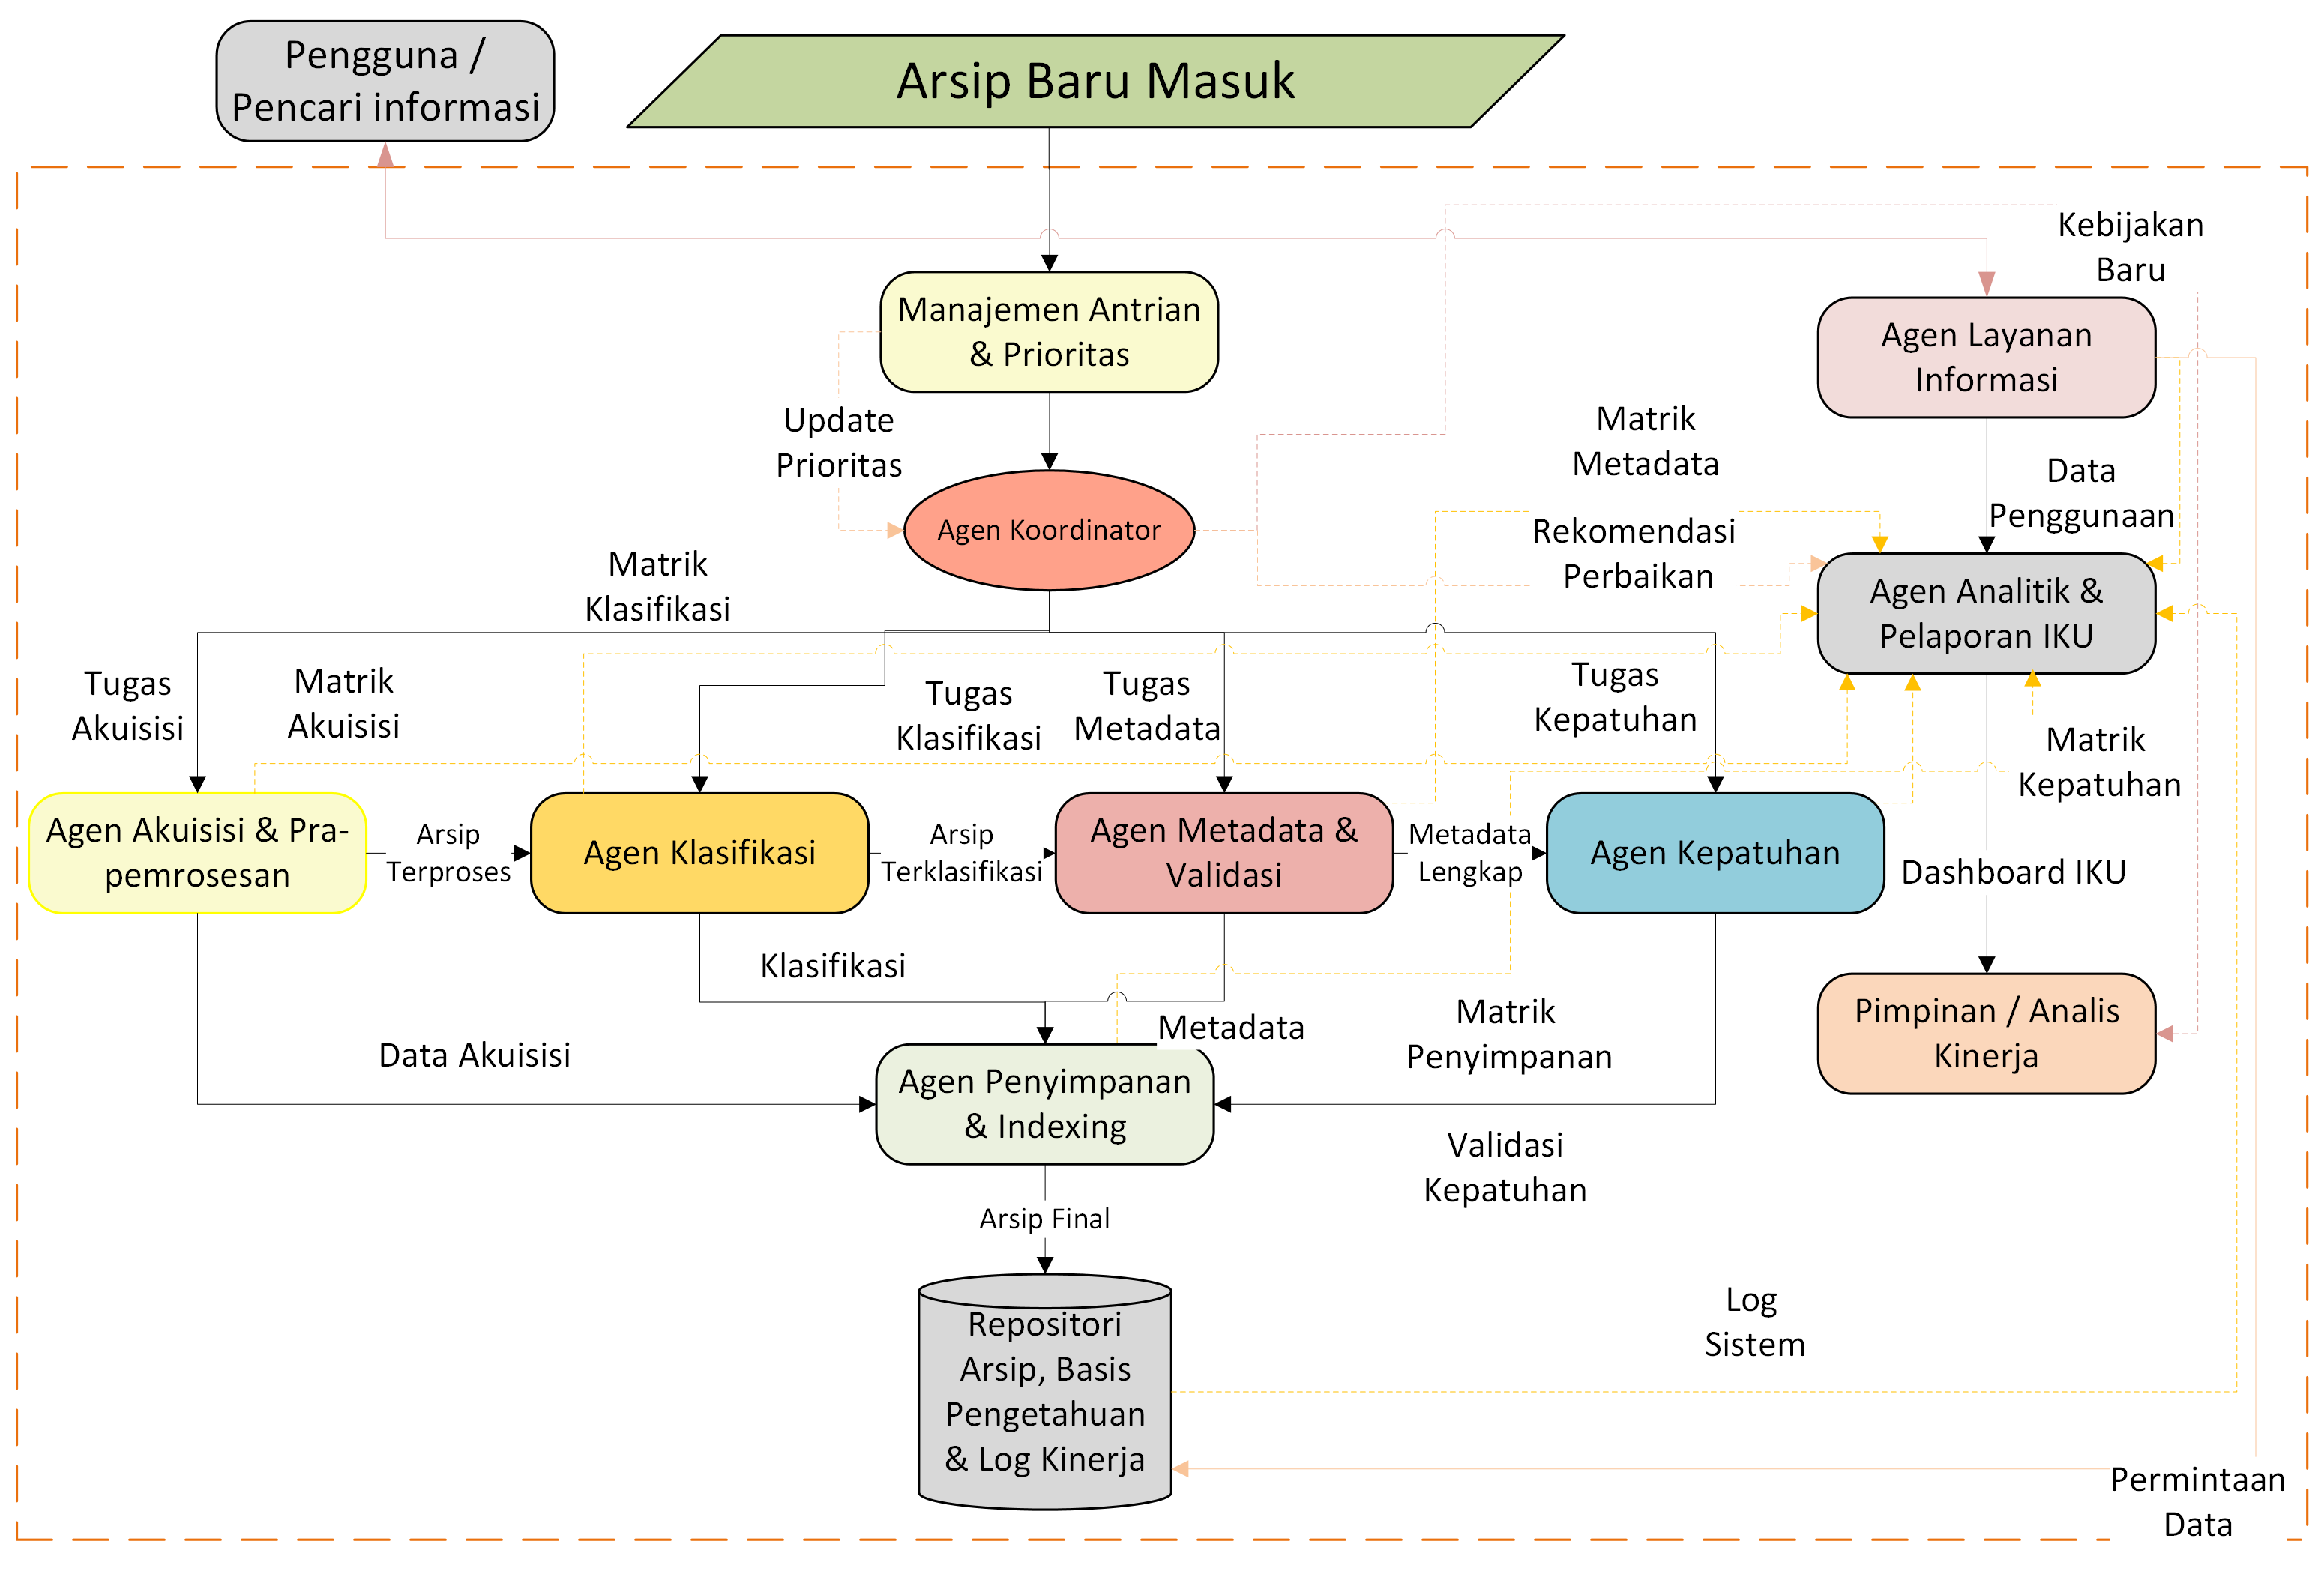
\includegraphics[width=2.9in,height=1.97222in]{media/media/image11.png}

Gambar 6. Model Konseptual Pemanfaatan Agentic AI dalam Tata Kelola
Kearsipan

Meskipun alurnya otomatis, sistem ini tetap mengintegrasikan peran
manusia melalui mekanisme \emph{Human-in-the-Loop} (HITL) pada
tahap-tahap kritis, seperti saat memvalidasi klasifikasi sensitif atau
memerlukan persetujuan disposisi. Di sepanjang proses ini, setiap agen
operasional secara aktif mengirimkan log aktivitas dan metrik kinerjanya
ke Agen Analitik \& Pelaporan IKU, yang berfungsi untuk memantau
kesehatan dan akuntabilitas sistem secara keseluruhan.

Agar seluruh alur kerja yang kompleks ini dapat berjalan secara cerdas
dan konsisten, sistem bergantung pada dua fondasi utama: repositori
arsip dan basis pengetahuan terpusat. Repositori arsip berfungsi sebagai
tempat penyimpanan utama untuk aset digital dan informasi lokasi arsip
fisik. Sementara itu, basis pengetahuan agen menjadi memori dari operasi
ini, yang berisi serangkaian aturan fundamental seperti skema
klasifikasi, standar metadata, JRA, serta kebijakan keamanan dan akses.
Basis pengetahuan ini juga dilengkapi dengan sumber daya pendukung
seperti tesaurus, model \emph{machine learning} untuk agen pembelajar,
dan rekam jejak sistem berupa log aktivitas yang terus diperbarui untuk
memandu setiap keputusan agen.

Model arsitektur Agentic AI yang diusulkan ini menyediakan kerangka
kerja untuk mendelegasikan tugas-tugas tata kelola data kearsipan kepada
entitas-entitas cerdas yang dapat bekerja secara otonom, proaktif, dan
terkoordinasi. Dengan mendefinisikan peran dan tanggung jawab yang jelas
untuk setiap agen, serta alur kerja yang terstruktur, model ini
berpotensi besar untuk meningkatkan konsistensi dalam penerapan
kebijakan, meningkatkan kualitas dan struktur metadata, serta secara
keseluruhan memperkuat efektivitas dan akuntabilitas tata kelola
kearsipan. Keberhasilan implementasi model ini akan bergantung pada
desain detail setiap agen, kualitas data dan aturan yang menjadi
inputnya, serta integrasi yang cermat dengan proses bisnis dan
intervensi manusia yang strategis.

\hypertarget{kesimpulan-saran}{%
\section{KESIMPULAN \& SARAN}\label{kesimpulan-saran}}

\textbf{5.1 Kesimpulan}

Penelitian ini menyimpulkan bahwa Agentic AI, yang diimplementasikan
melalui arsitektur Sistem Multi-Agen (MAS) yang terkoordinasi, memiliki
potensi signifikan untuk mentransformasi tata kelola data kearsipan.
Model yang diusulkan secara fundamental mengatasi tantangan terkait
inkonsistensi penerapan kebijakan dan kurangnya struktur metadata yang
sering terjadi pada sistem manual atau semi-otomatis. Dengan
mendelegasikan tugas-tugas inti seperti akuisisi, klasifikasi, ekstraksi
metadata, dan pemantauan kepatuhan kepada agen-agen cerdas yang bekerja
secara otonom dan proaktif, organisasi dapat mencapai tingkat
konsistensi, akurasi, dan efisiensi yang lebih tinggi dalam pengelolaan
arsip.

Selain solusi teknis, penelitian ini juga mengkaji tentang pergeseran
paradigma dalam tata kelola itu sendiri: dari kebijakan pasif menjadi
logika aktif yang terintegrasi. Dalam model ini, basis aturan atau basis
pengetahuan yang memuat skema klasifikasi, standar metadata, dan JRA
tidak lagi berfungsi sebagai dokumen rujukan, melainkan sebagai komponen
operasional yang secara langsung mengarahkan tindakan agen-agen AI. Agen
seperti Agen Klasifikasi dan Agen Kepatuhan secara konsisten
mengeksekusi aturan-aturan ini, memastikan kepatuhan secara desain
(\emph{compliance by design}) dan secara efektif meminimalkan risiko
yang timbul dari interpretasi manusia yang berbeda atau \emph{human
error}.

Sebagai hasil dari transformasi tata kelola ini, implementasi Agentic AI
diproyeksikan memberikan kontribusi positif dan terukur terhadap
pencapaian IKU kearsipan. Peningkatan IKU ini mencakup: (a) Ketersediaan
dan Aksesibilitas Arsip: Melalui otomasi proses pengolahan dan indexing
yang mempercepat waktu temu kembali informasi. (b) Kualitas Metadata:
Dengan otomatisasi ekstraksi, validasi kelengkapan, dan standardisasi
metadata yang menjadi tulang punggung sistem kearsipan yang andal. (c)
Efisiensi Layanan dan Kepatuhan: Melalui agen layanan cerdas yang
merespons permintaan rutin dan agen kepatuhan yang secara proaktif
memantau siklus hidup arsip sesuai regulasi.

\textbf{5.2 Saran}

Berdasarkan kesimpulan di atas, dirumuskan saran untuk pengembangan
penelitian selanjutnya dan rekomendasi praktis bagi institusi kearsipan.

Saran untuk Penelitian Selanjutnya: (a) Pengembangan Prototipe
Fungsional: Membangun prototipe dari arsitektur MAS yang diusulkan untuk
melakukan pengujian empiris terhadap kinerjanya, di luar cakupan
penelitian konseptual ini. Evaluasi dapat difokuskan pada metrik seperti
akurasi klasifikasi otomatis dan efisiensi alur kerja antar agen. (b)
Implementasi Studi Kasus: Menerapkan model pada lingkungan institusi
kearsipan nyata untuk mengidentifikasi faktor-faktor kontekstual,
tantangan implementasi praktis, dan dampak organisasional secara
mendalam. (c) Analisis Biaya-Manfaat: Melakukan analisis biaya-manfaat
yang komprehensif untuk mengkaji nilai investasi teknologi Agentic AI,
dengan membandingkan biaya implementasi terhadap keuntungan berupa
efisiensi operasional, pengurangan risiko, dan peningkatan kualitas
layanan.

Saran Praktis bagi Institusi Kearsipan: (a) Adopsi Paradigma Tata Kelola
sebagai Logika Aktif: Institusi harus memandang adopsi AI bukan sekadar
sebagai proyek otomatisasi tugas, melainkan sebagai kesempatan strategis
untuk mengoperasionalkan tata kelola. Langkah awal yang krusial adalah
memformalkan seluruh kebijakan dan aturan kearsipan menjadi format
terstruktur yang dapat dieksekusi oleh sistem. (b) Memulai dari Skala
Kecil (\emph{Pilot Project}): Mengimplementasikan solusi secara
bertahap. Fokus pada satu atau dua area yang paling mendesak dan
berdampak tinggi, seperti otomatisasi ekstraksi metadata untuk
mengurangi \emph{backlog} atau pemantauan JRA untuk mitigasi risiko. (c)
Pembangunan Kapasitas SDM: Mempersiapkan arsiparis dan pegawai untuk
beradaptasi dengan peran baru. Pelatihan harus difokuskan untuk mengubah
peran dari pelaksana manual menjadi supervisor sistem, validator dalam
skema HITL, dan analis data kinerja kearsipan.

\hypertarget{daftar-pustaka}{%
\section{DAFTAR PUSTAKA}\label{daftar-pustaka}}

Maurel, D., \& Zwarich, N. (2021). Information governance and power
relations: Reflections on archival education in Québec. \emph{Education
for Information}, \emph{37}(1), 33--51.
https://doi.org/10.3233/efi-190360

Luo, W., \& Hu, H. (2022). Analysis of the Path of Utilizing Big Data to
Innovate Archive Management Mode to Enhance Service Capability.
\emph{Wireless Communications and Mobile Computing}, \emph{2022}, 1--11.
https://doi.org/10.1155/2022/6207054

Tummers, J., Kassahun, A., \& Tekinerdogan, B. (2020). Reference
architecture design for farm management information systems: a
multi-case study approach. \emph{Precision Agriculture}, \emph{22}(1),
22--50. https://doi.org/10.1007/s11119-020-09728-0

Christiana, N., Helminasari, S., \& Pratama, P. Y. (2024).
Technology-Driven Archival Management in Samarinda's Library Service.
\emph{Indonesian Journal of Public Policy Review}, \emph{25}(3).
https://doi.org/10.21070/ijppr.v25i3.1401

Kerpedzhiev, G. D., König, U. M., Röglinger, M., \& Rosemann, M. (2020).
An Exploration into Future Business Process Management Capabilities in
View of Digitalization. \emph{Business \&amp; Information Systems
Engineering}, \emph{63}(2), 83--96.
https://doi.org/10.1007/s12599-020-00637-0

Colavizza, G., Blanke, T., Jeurgens, C., \& Noordegraaf, J. (2021).
Archives and AI: An Overview of Current Debates and Future Perspectives.
\emph{Journal on Computing and Cultural Heritage}, \emph{15}(1), 1--15.
https://doi.org/10.1145/3479010

Ma, N. (2024). Research on Archival Data Management in Local
Universities under the Context of Educational Informatization 2.0.
\emph{Philosophy and Social Science}, \emph{1}(4), 95--99.
https://doi.org/10.62381/p243414

Liu, Z. (2024). The Prospects and Challenges of Artificial Intelligence
Technology in Archival Management. \emph{Academic Journal of Management
and Social Sciences}, \emph{6}(3), 64--66.
https://doi.org/10.54097/wxdsk683

Miller, J., Davis‐Sramek, B., Fugate, B. S., Pagell, M., \& Flynn, B. B.
(2020). Editorial Commentary: Addressing Confusion in the Diffusion of
Archival Data Research. \emph{Journal of Supply Chain Management},
\emph{57}(3), 130--146. https://doi.org/10.1111/jscm.12236

Magnuson, J. A., Merrick, R., \& Case, J. T. (2020). Public Health
Information Standards. In \emph{Health Informatics} (pp. 129--145).
Springer International Publishing.
https://doi.org/10.1007/978-3-030-41215-9\_8

Jones, S. M., Klein, M., Weigle, M. C., \& Nelson, M. L. (2023).
Summarizing Web Archive Corpora via Social Media Storytelling by
Automatically Selecting and Visualizing Exemplars. \emph{ACM
Transactions on the Web}, \emph{18}(1), 1--48.
https://doi.org/10.1145/3606030

Indrasweri, N., Dwi Wahyuni, E. R., \& Rakhmawati, R. (2022).
Accessibility of Archival Reference Services. \emph{Record and Library
Journal}, \emph{8}(2), 199--206.
https://doi.org/10.20473/rlj.v8-i2.2022.199-206

Massihi, N., Abdolvand, N., \& Rajaee Harandi, S. (2020). A business
environment analysis model for renewable solar energy.
\emph{International Journal of Environmental Science and Technology},
\emph{18}(2), 401--416. https://doi.org/10.1007/s13762-020-02826-6

Tripathi, A. K., Agrawal, S., \& Gupta, R. D. (2020). Cloud enabled SDI
architecture: a review. \emph{Earth Science Informatics}, \emph{13}(2),
211--231. https://doi.org/10.1007/s12145-020-00446-9

Hosseini, S., \& Seilani, H. (2025). The role of agentic AI in shaping a
smart future: A systematic review. \emph{Array}, \emph{26}, 100399.
https://doi.org/10.1016/j.array.2025.100399

Sapkota, R., Roumeliotis, K. I., \& Karkee, M. (2025). \emph{AI Agents
vs. Agentic AI: A Conceptual Taxonomy, Applications and Challenges}
(Version 4). arXiv. https://doi.org/10.48550/ARXIV.2505.10468

Shinde, G., Kirstein, T., Ghosh, S., \& Franks, P. C. (2024). \emph{AI
in Archival Science -\/- A Systematic Review} (Version 1). arXiv.
https://doi.org/10.48550/ARXIV.2410.09086

Orkhan Masimov, Yashar Hajiyev, O. M., Yashar Hajiyev. (2024).
INTEGRATİON OF ARTİFİCİAL INTELLİGENCE (AI) İN TASK MANAGEMENT SYSTEMS.
\emph{PAHTEI-Procedings of Azerbaijan High Technical Educational
Institutions}, \emph{41}(06), 501--509.
https://doi.org/10.36962/pahtei41062024-55

Ackerman, L. (2025). \emph{Perceptions of Agentic AI in Organizations:
Implications for Responsible AI and ROI} (Version 1). arXiv.
https://doi.org/10.48550/ARXIV.2504.11564

Raza, S., Sapkota, R., Karkee, M., \& Emmanouilidis, C. (2025).
\emph{TRiSM for Agentic AI: A Review of Trust, Risk, and Security
Management in LLM-based Agentic Multi-Agent Systems} (Version 1). arXiv.
https://doi.org/10.48550/ARXIV.2506.04133
